%% For double-blind review submission, w/o CCS and ACM Reference (max submission space)
\documentclass[acmsmall,screen]{acmart}
% \settopmatter{printfolios=true,printccs=false,printacmref=false}
% \renewcommand\footnotetextcopyrightpermission[1]{} % removes footnote with conference information in first column
% \pagestyle{plain} % removes running headers

%% For double-blind review submission, w/ CCS and ACM Reference
%\documentclass[sigplan,review,anonymous]{acmart}\settopmatter{printfolios=true}
%% For single-blind review submission, w/o CCS and ACM Reference (max submission space)
%\documentclass[sigplan,review]{acmart}\settopmatter{printfolios=true,printccs=false,printacmref=false}
%% For single-blind review submission, w/ CCS and ACM Reference
%\documentclass[sigplan,review]{acmart}\settopmatter{printfolios=true}
%% For final camera-ready submission, w/ required CCS and ACM Reference
%\documentclass[sigplan]{acmart}\settopmatter{}


%%% If you see 'ACMUNKNOWN' in the 'setcopyright' statement below,
%%% please first submit your publishing-rights agreement with ACM (follow link on submission page).
%%% Then please update our instructions page and copy-and-paste the NEW commands into your article.
%%% Please contact us in case of questions; allow up to 10 min for the system to propagate the information.
%%%
%%% The following is specific to OOPSLA2 '22 and the paper
%%% 'Seq2Parse: Neurosymbolic Parse Error Repair'
%%% by Georgios Sakkas, Madeline Endres, Philip J. Guo, Westley Weimer, and Ranjit Jhala.
%%%
\setcopyright{rightsretained}
\acmPrice{}
\acmDOI{10.1145/3563330}
\acmYear{2022}
\copyrightyear{2022}
\acmSubmissionID{oopslab22main-p391-p}
\acmJournal{PACMPL}
\acmVolume{6}
\acmNumber{OOPSLA2}
\acmArticle{167}
\acmMonth{10}

%% Bibliography style
\bibliographystyle{ACM-Reference-Format}
%% Citation style
\citestyle{acmauthoryear}  %% For author/year citations
%\citestyle{acmnumeric}     %% For numeric citations
%\setcitestyle{nosort}      %% With 'acmnumeric', to disable automatic
                            %% sorting of references within a single citation;
                            %% e.g., \citep{Smith99,Carpenter05,Baker12}
                            %% rendered as [14,5,2] rather than [2,5,14].
%\setcitesyle{nocompress}   %% With 'acmnumeric', to disable automatic
                            %% compression of sequential references within a
                            %% single citation;
                            %% e.g., \citep{Baker12,Baker14,Baker16}
                            %% rendered as [2,3,4] rather than [2-4].


%%%%%%%%%%%%%%%%%%%%%%%%%%%%%%%%%%%%%%%%%%%%%%%%%%%%%%%%%%%%%%%%%%%%%%
%% Note: Authors migrating a paper from traditional SIGPLAN
%% proceedings format to PACMPL format must update the
%% '\documentclass' and topmatter commands above; see
%% 'acmart-pacmpl-template.tex'.
%%%%%%%%%%%%%%%%%%%%%%%%%%%%%%%%%%%%%%%%%%%%%%%%%%%%%%%%%%%%%%%%%%%%%%

%% Other packages
\usepackage{algorithm}
\usepackage[noend]{algpseudocode}
\usepackage{algorithmicx}
\usepackage{tikz}
\usetikzlibrary{positioning,shadows,arrows,trees,shapes,fit,patterns}
\usepackage{pgfplots}
\pgfplotsset{compat=1.12}
\usepackage{pgfplotstable}
\usepackage{bm}
\usepackage{framed}
\usepackage{amsmath}
% \usepackage{amssymb}
\usepackage{xspace}
\usepackage{listings}
\usepackage[skip=4pt]{caption}
\usepackage{wrapfig}
\usepackage{hyperref}
\usepackage[nameinlink,noabbrev]{cleveref}
\usepackage{multirow}
\usepackage{cite}

\lstset{
  language=Python,
  basicstyle=\small\ttfamily,
  keywordstyle=\small\ttfamily\bfseries,
  mathescape=true
}

\lstnewenvironment{ecode}{
\lstset{
  language=Python,
  basicstyle=\footnotesize\ttfamily,
  keywordstyle=\footnotesize\ttfamily\bfseries\color{deepblue},
  emphstyle=\footnotesize\ttfamily\bfseries\color{deepred},
  stringstyle=\footnotesize\ttfamily\color{deepgreen},
  literate=*
    {1}{{{\color{deepred}1}}}{1}
    {2}{{{\color{deepred}2}}}{1}
    {3}{{{\color{deepred}3}}}{1}
    {4}{{{\color{deepred}4}}}{1}
    {5}{{{\color{deepred}5}}}{1}
    {6}{{{\color{deepred}6}}}{1}
    {7}{{{\color{deepred}7}}}{1}
    {8}{{{\color{deepred}8}}}{1}
    {9}{{{\color{deepred}9}}}{1},
  numbers=left,
  xleftmargin=5.5mm,
  moredelim=[is][\bfseries]{==}{==},
  moredelim=[is][\underbar]{__}{__},
  moredelim=[is][\bfseries\underbar]{_=}{=_},
  escapeinside={(*@}{@*)}
}}
{}

\lstnewenvironment{rules}{
\lstset{
  language=Python,
  basicstyle=\footnotesize\ttfamily,
  keywordstyle=\footnotesize\ttfamily\bfseries,
  xleftmargin=0.5mm,
  numbers=none,
  moredelim=[is][\bfseries]{==}{==},
  moredelim=[is][\underbar]{__}{__},
  moredelim=[is][\bfseries\underbar]{_=}{=_},
  escapeinside={(*@}{@*)}
}}
{}

\MakeRobust{\Call}

\newcommand{\algorithmautorefname}{Algorithm}
\makeatletter
\renewcommand{\ALG@beginalgorithmic}{\small}
\renewcommand{\ALG@endalgorithmic}{\small}

% \renewcommand{\arraystretch}{1.1}
\makeatother

\lstMakeShortInline[language=Python, mathescape=true]{|}

%% Our commands
\usepackage{commands}

%% Some recommended packages.
\usepackage{booktabs}   %% For formal tables:
                        %% http://ctan.org/pkg/booktabs
\usepackage{subcaption} %% For complex figures with subfigures/subcaptions
                        %% http://ctan.org/pkg/subcaption


% This is the syntax highlighting for python:
\DeclareFixedFont{\ttb}{T1}{txtt}{bx}{n}{8} % for bold
\DeclareFixedFont{\ttm}{T1}{txtt}{m}{n}{8}  % for normal

% Custom colors
\definecolor{deepblue}{rgb}{0,0,0.5}
\definecolor{deepred}{rgb}{0.8,0,0}
\definecolor{deepgreen}{rgb}{0,0.5,0}

% Python style for highlighting
\newcommand\pythonstyle{\lstset{
language=Python,
basicstyle=\ttm,
morekeywords={self},              % Add keywords here
keywordstyle=\ttb\color{deepblue},
emph={MyClass,__init__},          % Custom highlighting
emphstyle=\ttb\color{deepred},    % Custom highlighting style
stringstyle=\color{deepgreen},
literate=*
  {1}{{{\color{deepred}1}}}{1}
  {2}{{{\color{deepred}2}}}{1}
  {3}{{{\color{deepred}3}}}{1}
  {4}{{{\color{deepred}4}}}{1}
  {5}{{{\color{deepred}5}}}{1}
  {6}{{{\color{deepred}6}}}{1}
  {7}{{{\color{deepred}7}}}{1}
  {8}{{{\color{deepred}8}}}{1}
  {9}{{{\color{deepred}9}}}{1},
frame=tb,                         % Any extra options here
showstringspaces=false
}}

% Python environment
\lstnewenvironment{python2}[1][]
{
\pythonstyle
\lstset{#1}
}
{}

% Python for external files
\newcommand\pythonexternal[2][]{{
\pythonstyle
\lstinputlisting[#1]{#2}}}

% Python for inline
\newcommand\pythoninline[1]{{\pythonstyle\lstinline!#1!}}



\begin{document}

%% Title information
\title[\toolname]{\toolname: Neurosymbolic Parse Error Repair}

% \titlenote{with title note}             %% \titlenote is optional;
%                                         %% can be repeated if necessary;
%                                         %% contents suppressed with 'anonymous'
% \subtitle{Subtitle}                     %% \subtitle is optional
% \subtitlenote{with subtitle note}       %% \subtitlenote is optional;
%                                         %% can be repeated if necessary;
%                                         %% contents suppressed with 'anonymous'
%% Author information
%% Contents and number of authors suppressed with 'anonymous'.
%% Each author should be introduced by \author, followed by
%% \authornote (optional), \orcid (optional), \affiliation, and
%% \email.
%% An author may have multiple affiliations and/or emails; repeat the
%% appropriate command.
%% Many elements are not rendered, but should be provided for metadata
%% extraction tools.

%% Author with single affiliation.
\author{Georgios Sakkas}
% \authornote{with author1 note}          %% \authornote is optional;
%                                         %% can be repeated if necessary
% \orcid{nnnn-nnnn-nnnn-nnnn}             %% \orcid is optional
\affiliation{
  % \position{Position1}
  \department{Computer Science \& Engineering}
  \institution{University of California, San Diego}
  % \streetaddress{Street1 Address1}
  \city{La Jolla}
  \state{CA}
  % \postcode{Post-Code1}
  \country{USA}
}
\email{gsakkas@eng.ucsd.edu}

\author{Madeline Endres}
\affiliation{
  \department{Computer Science \& Engineering}
  \institution{University of Michigan}
  \city{Ann Arbor}
  \state{MI}
  \country{USA}
}
\email{endremad@umich.edu}

\author{Philip J. Guo}
\affiliation{
  \department{Computer Science \& Engineering}
  \institution{University of California, San Diego}
  \city{La Jolla}
  \state{CA}
  \country{USA}
}
\email{pg@ucsd.edu}

\author{Westley Weimer}
\affiliation{
  \department{Computer Science \& Engineering}
  \institution{University of Michigan}
  \city{Ann Arbor}
  \state{MI}
  \country{USA}
}
\email{weimerw@umich.edu}

\author{Ranjit Jhala}
\affiliation{
  \department{Computer Science \& Engineering}
  \institution{University of California, San Diego}
  \city{La Jolla}
  \state{CA}
  \country{USA}
}
\email{jhala@cs.ucsd.edu}

\begin{abstract}
We present \toolname, a language-agnostic neurosymbolic approach to
automatically repairing parse errors.
%
\toolname is based on the insight that
%
\emph{Symbolic} Error Correcting (EC) Parsers can, in principle,
synthesize repairs, but, in practice, are overwhelmed by
the many error-correction rules that are not \emph{relevant}
to the particular program that requires repair.
%
In contrast, \emph{Neural} approaches are fooled by the large
space of possible sequence level edits, but can precisely
pinpoint the set of EC-rules that \emph{are} relevant
to a particular program.
%
We show how to combine their complementary strengths
by using neural methods to train a sequence classifier
that predicts the small set of relevant EC-rules
for an ill-parsed program, after which, the symbolic
EC-parsing algorithm can make short work of generating
useful repairs.
%
We train and evaluate our method on a dataset of 1,100,000
Python programs, and show that \toolname is
%
\emph{accurate} and \emph{efficient}: it can parse $94\%$
of our tests within $2.1$ seconds, while generating the
exact user fix in 1 out 3 of the cases; and
%
\emph{useful}: humans perceive both \toolname-generated error locations and
repairs to be almost as good as human-generated ones in a
statistically-significant manner.
\end{abstract}


%% 2012 ACM Computing Classification System (CSS) concepts
%% Generate at 'http://dl.acm.org/ccs/ccs.cfm'.
\begin{CCSXML}
  <ccs2012>
    <concept>
        <concept_id>10011007.10011006.10011039.10011040</concept_id>
        <concept_desc>Software and its engineering~Syntax</concept_desc>
        <concept_significance>300</concept_significance>
        </concept>
    <concept>
        <concept_id>10010147.10010257</concept_id>
        <concept_desc>Computing methodologies~Machine learning</concept_desc>
        <concept_significance>300</concept_significance>
        </concept>
    <concept>
        <concept_id>10011007.10011006.10011041.10011688</concept_id>
        <concept_desc>Software and its engineering~Parsers</concept_desc>
        <concept_significance>500</concept_significance>
        </concept>
    <concept>
        <concept_id>10011007.10011074.10011092.10011782</concept_id>
        <concept_desc>Software and its engineering~Automatic programming</concept_desc>
        <concept_significance>500</concept_significance>
        </concept>
    <concept>
        <concept_id>10002950.10003648.10003671</concept_id>
        <concept_desc>Mathematics of computing~Probabilistic algorithms</concept_desc>
        <concept_significance>300</concept_significance>
        </concept>
  </ccs2012>
\end{CCSXML}

\ccsdesc[300]{Software and its engineering~Syntax}
\ccsdesc[300]{Computing methodologies~Machine learning}
\ccsdesc[500]{Software and its engineering~Parsers}
\ccsdesc[500]{Software and its engineering~Automatic programming}
\ccsdesc[300]{Mathematics of computing~Probabilistic algorithms}
%% End of generated code


%% Keywords
%% comma separated list
\keywords{Automated Program Repair, Machine Learning, Error-Correcting Parsers}  %% \keywords are mandatory in final camera-ready submission


%% \maketitle
%% Note: \maketitle command must come after title commands, author
%% commands, abstract environment, Computing Classification System
%% environment and commands, and keywords command.
\maketitle

\section{Introduction}
\label{sec:intro}

% Context
Writing syntactically-correct code can be difficult for novice 
programmers. Consider the simple program,
shown in \autoref{fig:bad-prog}, which defines two functions |foo| and
|bar|. 
% Function |foo| adds the argument variable |a| and returns
% it. Function |bar| calls |foo| with the argument variable |a|, adds another
% number and returns the result. 
The programmer has introduced an extra |+| operator after the
|return b| statement on line 6. This extra |+| likely needs to be deleted, as the
programmer intended in the fixed program in \autoref{fig:fixed-prog}. This
example presents a \emph{syntax} (or \emph{parse}) \emph{error}. Such parse errors can easily
go unnoticed~\citep{Denny_2012, Ahadi_2018} by programmers when they are part of
bigger programs and may require significant effort to fix~\citep{Kummerfeld2003}.

% Our goal is to use historical data of how programmers have fixed similar errors
% in their programs to automatically and rapidly guide programmers to come up with
% candidate solutions like the one above.

\begin{figure}[h]
\centering
\begin{minipage}[c]{0.48\linewidth}
\begin{ecode}
def foo(a):
  return a + 42

def bar(a):
  b = foo(a) + 17
  return b +
\end{ecode}
\subcaption{A Python program with two functions that manipulate an integer. The second one has a parse error.}
\label{fig:bad-prog}
\end{minipage}%
\hspace{0.02\linewidth}%
\begin{minipage}[c]{0.48\linewidth}
\begin{ecode}
def foo(a):
  return a + 42

def bar(a):
  b = foo(a) + 17
  return b
\end{ecode}
\subcaption{A possible fixed version for the previous example that has no parse
 errors.}
\label{fig:fixed-prog}
\end{minipage}
\caption{A simple Python program example}
\label{fig:example-prog}
\end{figure}

% Gap
\emph{Parsing algorithms}, which check compliance with syntax rules, are
essential parts of programming systems. Research around these algorithms
has led to 
efficient or expressive parsers used in modern programming languages, \eg 
LR parsing~\citep{Aho1974} or Earley parsing~\citep{Earley_1970}. These highly-engineered
approaches are usually very accurate in locating syntax errors, however, many
times they fail to provide effective feedback to the developers. For example, they may only
point to the first syntax error or may produce messages that are not descriptive enough
or are too verbose~\citep{Kummerfeld2003, Ahadi_2018,
VanDerSpek_2005}. 
% WRW doesn't understand this claim and does not think it is true without
% more explanation. GCC is push-button, requiring no SE effort. 
% 
% Additionally, these parsers require a lot of manual effort from the software engineers.

Recent advances in the Natural Language Processing (NLP) research domain
\citep{Sutskever_2014, Hardalov_2018} have suggested many automatic approaches
for natural language applications, such as language translation. In
particular, \emph{sequence models} can learn underlying
patterns in their data and have been shown to be remarkably
effective at parsing \citep{Vinyals2015}. The vast availability of data has
rendered such deep neural network (\dnn) architectures rather successful. They
are able to learn to effectively parse sentences into their associated
(serialized) parse trees. Such approaches have been considered for
automatically parsing and repairing programs~\citep{Ahmed_2021}, but 
initial efforts lacked accuracy in real-world contexts. 

In programming languages research, \emph{error
correcting parsers} (EC-Parsers) \citep{Aho_1972} use special error production
rules to support parsing programs with syntax errors. These parsers can return
minimal-edit repairs that make the programs parse and can simultaneously fix
multiple locations with minimal effort from the programmers. Their drawback,
however, is that they have a cubic time complexity with respect to the
input program size and a quadratic complexity with respect to the grammar
used. 
% WRW doesn't see why this next bit is a problem the reader cares about. It
% seems like an internal issue that has the same symptom (bad complexity)
% and is more like "our problem". 
% 
% Futhermore, there is the added cost of the
% large number of additional production rules these parsers have to consider while
% having an explosion of the internal states by maintaining the cost of each
% possible parse. 
Unfortunately, these scalability issues have remained over the
decades~\citep{McLean1996, Rajasekaran2014}, leaving EC-Parsers
impractical for most uses in real-world programming languages.

% Innovation
\mypara{Sequence Classifiers for Error-Correcting Parsing}
In this work, we propose training sequence classifiers for predicting error
production rules for EC-Parsers in order to automatically, accurately and
efficiently parse programs with syntax errors. Our approach exploits data-driven
approaches from sequence learning and realizes them by using a large training
dataset of pairs of syntactically incorrect programs and their fixed versions.
%
Specifically, to enable the efficient usage of a scalable EC-Parser we decompose
the problem into three steps:
%
First, \emph{learn} the set of error productions rules that fix the dataset of
programs from a corpus of fix edits that the users made.
%
Second, \emph{predict} the small set of error rules for a new erroneous program,
by training sequence multi-class classifiers on abstracted program token
sequences.
%
Third, \emph{parse} the given erroneous program with the predicted error rules,
thus generating a repair.
%
Critically, we show how to perform the crucial abstraction from a particular
program to an abstract token sequence by using an Earley parser's
\citep{Earley_1970} partial parses and a learnt Probabilistic Context-Free
Grammar. This abstraction lets us train accurate predictors over low-level
program sequences allowing the efficient error-correcting parsing of programs
with syntax errors.

% Results
\mypara{\toolname}
We implemented our approach in \toolname and trained it and tested it on a
dataset of more than 1,100,000 programs. Given a new erroneous program,
\toolname generates a list of potential error production rules ranked by
likelihood. We train \toolname on programs from a online editor from over two
years and evaluate in several ways.
%
First, we measure its \emph{accuracy}: we show that \toolname correctly predicts
the right set of error rules $81\%$ of the time when considering the top $20$
rules and can parse $92\%$ of our tests within $4.1$ seconds with these
predictions.
%
Second, we measure its \emph{efficiency}: we show that \toolname is able to
parse and repair erroneous programs within $25$ seconds $81\%$ of the time,
while also generating \emph{the user fix in almost 1 out 3 of the cases}.
%
Finally, we measure the \emph{quality} of the generated repairs via a user study
with XX participants and show that humans perceive both \toolname's edit
locations and final repair quality to be better than YY in a
statistically-significant manner.

\section{A Case for Parse Error Repair}
\label{sec:error-analysis}

We motivate \toolname by analyzing a dataset
comprising \emph{1,100,000 erroneous Python programs}
and their respective fixes.
%
This dataset was gathered from PythonTutor.com~\citep{Guo2013}
between the years 2017 and 2018, previously used in related
work~\citep{Endres2019, Cosman2020}.
%
Each program which throws an uncaught \python exception
is paired with the next program by the same user that does
not crash, under the assumption that the latter is the fixed
version of the former.
%
We discard pairs that are too different between buggy
and fixed versions, since these are usually unrelated
submissions or complete refactorings.
%
We also discard submissions that violate PythonTutor's
policies (\eg, those using forbidden libraries).
%
The resulting dataset contains usable program pairs,
representing students from dozens of universities
(PythonTutor has been used in many introductory
courses~\citep{Guo2013}) as well as non-traditional
novices.

\begin{figure}[t]
  \centering
  \begin{minipage}[c]{0.48\linewidth}
    \centering
    \includegraphics[width=\linewidth]{error-pie.pdf}
    \caption{The Python error type distribution.}
    \label{fig:error-statistics}
  \end{minipage}
  \hspace{0.02\linewidth}
  \begin{minipage}[c]{0.48\linewidth}
      \centering
      \includegraphics[width=\linewidth]{fixed-rate.pdf}
      \caption{The repair rates of the Python dataset.}
      \label{fig:repair-rate}
  \end{minipage}
\end{figure}

One might imagine that parse (or \emph{syntax}) errors are
usually easier to locate and repair than other algorithmic
or runtime errors \citep{Denny_2012}.
%
For example, the Python parser will immediately inform the programmer
about missing parentheses in function argument lists or for not having
the proper indents in a statement block.
%
However, as has also been shown in previous
work \citep{Ahadi_2018, Kummerfeld2003}, our
data confirms that programmers (especially novices)
deal with these kinds of errors regularly and
spend a considerable amount of time fixing them.

\mypara{Observation 1: Parse errors are very common}
%
\autoref{fig:error-statistics} presents the statistics
of the different types of errors that users encountered
in this dataset.
%
We observe that $77.4 \% $ of all faulty programs failed
with a syntax error, accounting for the vast majority of
the errors that (novice) programmers face with their
programs.
%
The second category is merely $13.6\%$ of the dataset and
represents Python type errors. This is a strong indication
that parse errors are a very common type of error.

\mypara{Observation 2: Parse errors take time to fix}
%
The web-based compiler that we used to generate this
dataset provides us with a \emph{server timestamp}.
%
The timestamp is associated with each program attempt
submission, erroneous or not. The \emph{repair time}
of an erroneous program is calculated by taking the
difference of the two timestamps of the erroneous and
fixed program.
%
This method can be an inaccurate metric of repair time,
as there are various reasons these timings may be exaggerated,
\eg users stepping away from the computer, internet lag \etc.
%
However, in aggregate, due to the large
dataset of program repairs, these timings
can still be viewed as an approximate metric
of the amount of time it took novice programmers to
repair their program errors.

\autoref{fig:repair-rate} shows the \emph{programmer repair rate},
\ie the dataset percentage that is repaired under a given amount of time.
%
It presents the repair rate for parse errors and the rest
of the error types, grouped together here as \emph{runtime} errors.
%
As expected, parse errors are fixed faster than the rest,
but \emph{not by a large difference}.
%
For example, we observe that within 2 minutes,
usually $46\%$ of the runtime errors are repaired, while
around $63\%$ of the syntax errors are.
%
Although, this is a considerable difference,
we observe that there is still a large number
of the ``simpler'' parse errors that required
more than 2 minutes to be fixed.

\begin{figure}[t]
  \centering
  \begin{minipage}[c]{0.48\linewidth}
    \centering
    \includegraphics[width=\linewidth]{dataset-ratio-per-change.pdf}
    \caption{The Python dataset ratio that is fixed under the given number of
     token changes.}
    \label{fig:token-changes-ratio}
  \end{minipage}
  \hspace{0.02\linewidth}
  \begin{minipage}[c]{0.48\linewidth}
      \centering
      \includegraphics[width=\linewidth]{median-repair-times.pdf}
      \caption{The average time the user needed to fix the erroneous program
      for the needed token changes.}
      \label{fig:token-changes}
  \end{minipage}
\end{figure}

\mypara{Observation 3: Parse errors may need multiple edits to fix}
%
The average \emph{token-level changes} needed to fix a program with syntax
errors, \ie the number of changes in the lexed program token sequence, is
\emph{10.7 token changes}, while the \emph{median is 4}.
%
A variable rename or a different integer are not considered as changes
as they won't affect the syntax error fix.
%
As shown in \autoref{fig:token-changes-ratio}, $14.2\%$ of errors
need only 1 token change, $23.2\%$ need 2 token changes, $7.0\%$
need 3 and $9.0\%$ need 4.
% Ultimately, $53.4\%$ of these errors needs at most 4 token changes to be fixed.
Ultimately, $46.6\%$ of these errors require more than 4 token changes.
%
% It is also important to see how long it takes the users on average to make
% those changes.

\mypara{Observation 4: Parse errors with more edits take longer to fix}
%
\autoref{fig:token-changes} shows the average time that it takes a user to fix
all of their syntax errors per the number of token-level changes in their
programs. As expected, with an increasing number of token changes needed,
programmers need more time to implement those changes. Most importantly, even
for 1 or 2 token changes the average user spends \emph{26 and 25 sec}
respectively, which is still a considerable amount of time for such simple and
short fixes. The repair time jumps to \emph{56 sec} for three token changes.

\smallskip
These four observations indicate that, while some errors can be
easily and quickly fixed by programmers using existing error messages,
there are many cases where novices struggle with fixing syntax errors.
%
Therefore, we can conclude that an automated tool that parses and repairs
such programs in only a few seconds could benefit many novices.

\section{Overview}
\label{sec:overview}

We begin with an overview of our approach to suggesting fixes for programs with
parse errors by fine-tuning error correcting parsers with prior knowledge of the
processes (novice) programmers follow to repair their errors.

\begin{figure}[h]
\centering
\begin{minipage}[c]{0.48\linewidth}
\begin{ecode}
def foo(a):
  return a + 42

def bar(a):
  b = foo(a)
  return b +
\end{ecode}
\subcaption{A Python program with two functions that manipulate an integer,
where the second one has a parse error.}
\label{fig:bad-prog}
\end{minipage}%
\hspace{0.02\linewidth}%
\begin{minipage}[c]{0.48\linewidth}
\begin{ecode}
def foo(a):
  return a + 42

def bar(a):
  b = foo(a)
  return b + 17
\end{ecode}
\subcaption{A possible fixed version for the previous example that has no parse
 errors.}
\label{fig:fixed-prog}
\end{minipage}
\caption{A simple Python program example}
\end{figure}


\mypara{The Problem} Consider the simple program shown in
\autoref{fig:bad-prog}. The program defines two functions \texttt{foo} and
\texttt{bar}. Function \texttt{foo} adds some number to the argument variable
\texttt{a} and returns it. Function \texttt{bar} calls \texttt{foo} with the
argument variable \texttt{a} and returns the result. However, there is an extra
\texttt{+} operator after the \texttt{return} statement. The extra \texttt{+}
can either be deleted or the programmer most likely intended to add another
number like the fix shown in the bottom of \autoref{fig:fixed-prog}. This is a
\emph{syntax or parse error} and such parse errors can easily go unnoticed
\citep{Denny_2012, Ahadi_2018, VanDerSpek_2005} by programmers when they are
part of bigger programs. Our goal is to use historical data of how programmers
have fixed similar errors in their programs to automatically and rapidly guide
programmers to come up with candidate solutions like the one above.


\mypara{Solution: Error Correcting Parsers}
One approach to make such erroneous programs parse is to use \emph{Error
Correcting Parsers} (EC-Parsers) \citep{Aho_1972}. EC-Parsers are based on
\emph{dynamic programming algorithms} and have been used in recent literature to
automatically infer the intended parse tree for a program that doesn't belong to
a certain programming language, \ie a program that has a syntax error. These
dynamic programming parsers have been used along side with \emph{error
correcting production rules} \citep{Aho_1972} to generate a valid parse by
making minimal edits to the original program.

\mypara{Another Problem}
However, these error-correcting parsers have a time complexity that is cubed on
the input program size and squared on the grammar size used. Futhermore, there
is the added cost of the large number of additional production rules these
parsers have to consider while having an explosion of the internal states by
maintaining the cost of each possible parse. Therefore, they are not tractable
or scalable options for real-world programming languages and programs.


\mypara{Solution: Train classifier to predict error rules}
The original Earley parsing is a fairly efficient parsing algorithm
\citep{Earley_1970} based on dynamic programming. Its error-correcting version
becomes very inefficient though for larger real-world grammars, since it
requires the addition of a large number of error production rules as mentioned
before. However, not every erroneous program needs all of those rules to be
parsed. In this work, we present a novel strategy to selecting just a small set
of error production rules that can be used with an updated \emph{Error
Correcting Earley Parser} (ECE-Parser) to repair a program with parse errors.
%
To enable the efficient usage of a scalable ECE-Parser we decompose the problem into 3
steps:
%
First, \emph{learn} the set of error productions rules each program with a parse
error needs from a corpus of fixed programs.
%
Second, \emph{predict}, for each erroneous program, a small set of error rules.
%
Third, \emph{parse} an erroneous program with the predicted rules and generate a
fix.
%
In the remainder of this section, we give a high-level overview
of our approach by describing how to:

\begin{enumerate}

  \item Use an \emph{Error Correcting Earley Parser} (ECE-Parser) to repair programs
  with parse errors (\S~\ref{sec:overview:ec-parsing}),

  \item Abstract erroneous programs with their \emph{partial parses} by using
  Probabilistic Context-Free Grammars (PCFGs)
  (\S~\ref{sec:overview:abstraction}),

  \item Train \emph{sequence classifiers} on the abstracted programs to predict
  small sets of error production rules (\S~\ref{sec:overview:train}).

\end{enumerate}

\subsection{Error Correcting Parsing}
\label{sec:overview:ec-parsing}

\begin{figure}[t]
\begin{ecode}
S        (*@$\rightarrow$@*) Stmts end_marker
Stmts    (*@$\rightarrow$@*) Stmt \n | Stmt \n Stmts
Stmt     (*@$\rightarrow$@*) FuncDef | ExprStmt | RetStmt | PassStmt | ...
FuncDef  (*@$\rightarrow$@*) def name Params : Block
Block    (*@$\rightarrow$@*) \n indent Stmts dedent
RetStmt  (*@$\rightarrow$@*) return | return Args
Args     (*@$\rightarrow$@*) ExprStmt | ExprStmt , Args
ExprStmt (*@$\rightarrow$@*) ArExpr | ...
ArExpr   (*@$\rightarrow$@*) Literal | ArExpr BinOp Literal
Literal  (*@$\rightarrow$@*) name | number | ...
...
\end{ecode}
\caption{Simplified production rules of the Python grammar}
\label{fig:production-rules}
\end{figure}

\mypara{Earley Parsing and Grammars} Earley parsing has been a touch-stone
algorithm in the history of parsing \citep{Earley_1970}. An Earley parser is a
\emph{top-down chart parser} that uses dynamic programming, meaning that partial
parses are stored in a data structure called a \emph{chart}, which can later be
re-used, and the parse tree is built from the top down. An (Earley) parser
accepts programs that belong into a language that is defined by a given
\emph{grammar} $G$. A grammar has a starting symbol \texttt{S} and a set of
\emph{production rules}. \autoref{fig:production-rules} presents some simplified
production rules for the Python language that will help parse the program in
\autoref{fig:bad-prog}. \emph{Terminal} symbols (or \emph{tokens}) are symbols
that a Python program consists of and are presented here in lowercase letters.
Symbols that start with a capital letter here represent \emph{non-terminal}
symbols. For example, the non-terminal \texttt{Stmt} defines all the possible
Python statements, \ie expressions (\texttt{ExprStmt}), return statements
(\texttt{ReturnStmt}), \etc

\begin{figure}
    \centering
    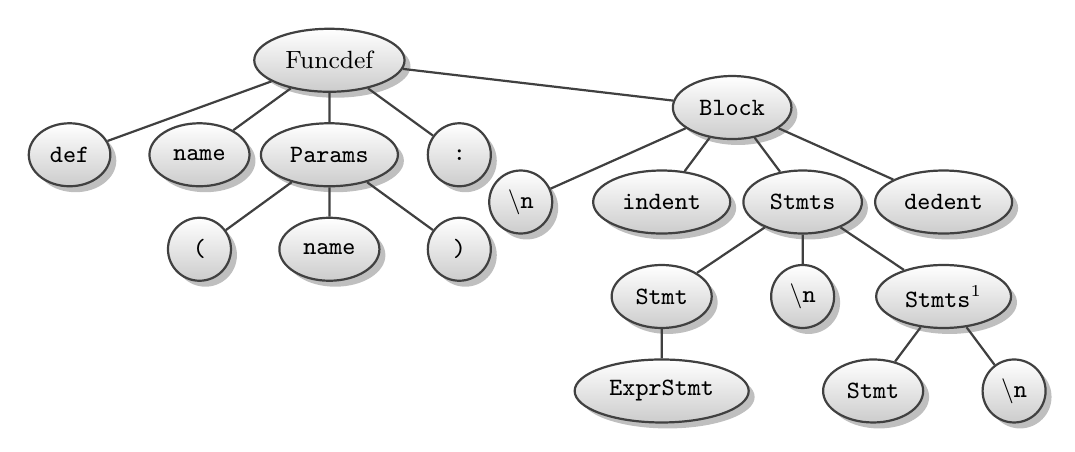
\begin{tikzpicture}
    [font=\small, edge from parent,
    every node/.style={top color=white, bottom color=black!20,
    ellipse, minimum size=8mm, draw=black!75,
    thick, drop shadow, align=center},
    edge from parent/.style={draw=black!75, thick},
    level distance=1.2cm, xscale=1.1]
    \node (func) {Funcdef}
        child {
            node (def) {\texttt{\bfseries def}}
        }
        child {
            node (name1) {\texttt{name}}
        }
        child {
            node (params) {\texttt{Params}}
            child {
                node (openParen) {\texttt{\bfseries (}}
            }
            child {
                node (name2) {\texttt{name}}
            }
            child {
                node (closeParen) {\texttt{\bfseries )}}
            }
        }
        child {
            node (colon) {\texttt{\bfseries :}}
        }
        child [level distance=0.6cm, xscale=1.55] {
            node (block) {\texttt{Block}}
            child [level distance=1.2cm, xscale=0.7] {
                node (newline1) {\texttt{\textbackslash n}}
            }
            child [level distance=1.2cm, xscale=0.7] {
                node (indent) {\texttt{indent}}
            }
            child [level distance=1.2cm, xscale=0.7] {
                node (stmts1) {\texttt{Stmts}}
                child {
                    node (stmt1) {\texttt{Stmt}}
                    child {
                        node (expr1) {\texttt{ExprStmt}}
                    }
                }
                child {
                    node (newline2) {\texttt{\textbackslash n}}
                }
                child {
                    node (stmts2) {\texttt{Stmts$^1$}}
                    child {
                        node (stmt2) {\texttt{Stmt}}
                    }
                    child {
                        node (newline3) {\texttt{\textbackslash n}}
                    }
                }
            }
            child [level distance=1.2cm, xscale=0.7] {
                node (dedent) {\texttt{dedent}}
            }
        };
    \end{tikzpicture}
    \caption{The partial parse tree generated for the example at
    \autoref{fig:bad-prog}}
    \label{fig:partial-parse-tree-1}
\end{figure}

%
% \begin{figure}[t]
% \begin{ecode}
% New_S     -> S | S Insert
% ...
% Block     -> E_\n E_indent Stmts E_dedent
% RetStmt   -> ... | E_return | E_return Args
% ...
% E_return  -> return | (*@$\epsilon$@*) | Replace | Insert return
% E_number  -> number | (*@$\epsilon$@*) | Replace | Insert number
% E_\n      -> \n | (*@$\epsilon$@*) | Replace | Insert \n
% ...
% Replace   -> return | pass | \n | ... [all terminals]
% Insert    -> Token | Insert Token
% Token     -> return | pass | \n | ... [all terminals]
% \end{ecode}
% \caption{Error production rules for the simplified Python grammar presented in
% \autoref{fig:production-rules}}
% \label{fig:error-rules}
% \end{figure}

\mypara{Error Correcting Parsing} Recent work has presented an \emph{Error
Correcting Earley Parser} (ECE-Parser) \citep{Aho_1972}, which extends the
original algorithm's operations, with the goal to find a minimum-edit parse for
a program with parse errors. An ECE-Parser extends the original grammar $G$ with
a set of \emph{error production rules} to create a new \emph{error grammar}
$G'$. This grammar contains error rules for three major types of errors that the
ECE-Parser considers, \ie it adds error rules that account for \emph{insertion},
\emph{deletion}, \emph{replacement} errors.

First of all, the ECE-Parser adds a new start symbol |New_S|, the helper symbol
|Replace| that is used for replacement errors and the symbols |Insert| and
|Token| that introduce insertion errors. Additionally, for each terminal |t| it
adds the new non-terminal |E_t| that introduces errors relevant to the |t|
symbol.

Next, in addition to the existing production rules, the error grammar $G'$ has
the following error rules. The new start symbols uses the old one with the
option of an insertion error at the end:
\begin{itemize}
  \item \lstinline{New_S  -> S | S Indent}
\end{itemize}
Also, for each non-terminal |T| it adds some non-terminal error rules that
introduce the terminal errors when the parsing algorithm is executed. For
example, the |Block| and |RetStmt| rules are updated as:
\begin{itemize}
  \item \lstinline{Block    -> ... | E_\n E_indent Stmts E_dedent}
  \item \lstinline{RetStmt  -> ... | E_return | E_return Args}
\end{itemize}
Next, for each terminal |t|, we add four error rules of the type:
\begin{itemize}
  \item \lstinline{E_t -> t | $\epsilon$ | Replace | Insert t}
\end{itemize}
These four new error rules has the following usage for each terminal |t|:
\begin{enumerate}
  \item The |E_t -> t| rule will match the original terminal |t| without any
  errors. This error rule is used in cases that the \emph{non-error} version of
  the rule is needed. For example, in \break
  |Block -> E_\n E_indent Stmts E_dedent| it can be the case that only
  |E_dedent| is needed to match the error and |E_\n| and |E_indent| can match
  their respective symbols.
  \item Using |E_t ->| $\epsilon$ a \emph{deletion} error is considered. The
  error rule will match \emph{nothing} or the \emph{empty token} $\epsilon$ in
  the program, meaning the terminal is missing.
  \item Using |E_t -> Replace| a \emph{replacement} error is considered.
  |Replace| will match any terminal token that is \emph{different} than |t|,
  making a replacement possible.
  \item  The rules |E_t -> Insert t| will introduce a \emph{insertion} error,
  \ie |Insert| will match any \emph{sequence} of |Token|s that are not supposed
  to precede |t| in order to make the program parse.
\end{enumerate}
% When, for example, a \texttt{Return\_Stmt} is added to the ECE-Parser's chart at
% some location $i$, then the next four options are considered:
% \begin{enumerate}
%   \item There is a \texttt{\bfseries return} at location $i+1$ of the tokenized
%   program and therefore the original \emph{non-error} production rules are used
%   to and are added to the chart at location $i+1$.
%   \item An \emph{insertion} error is considered, \ie there is a token at program
%   location $i$ that doesn't match any of the production rules. Then
%   \texttt{Err\_Return -> H return} is used to introduce one or more of these
%   insertion errors together with the rules \texttt{H -> H \textbar\ H Insert}
%   and \texttt{Insert -> \textbf{pass} \textbar\ \textbf{raise} \textbar\
%   \textbf{return} \textbar\ ...}. When \texttt{Insert} will match an
%   extraneous token $t$ in the program, then $t$ will be ignored in the final
%   parse repair.
%   \item A \emph{deletion} error is considered when an incomplete non-terminal
%   production rule is in the chart at location $i$ and the next symbol is a
%   terminal in the rule but is not present in the token sequence. Then
%   \texttt{Err\_Return -> e} is used to match an \emph{empty} token. At the final
%   stage, the relevant terminal (here a \texttt{\textbf{return}}) will be added
%   at location $i+1$ to generate a repaired program.
%   \item A \emph{replacement} error is considered here when an incomplete
%   non-terminal production rule is in the chart at location $i$ and the next
%   symbol is a terminal in the rule but is not the same in the token sequence.
%   Then \texttt{Err\_Return -> Err\_Tag} is used to match the program token $t$.
%   At the final stage, the relevant terminal (here a \texttt{\textbf{return}})
%   will replace the program token $t$.
% \end{enumerate}

For example, for the terminal tokens |return|, |number| and |\n| (a new line)
the relevant error production rules are:
\begin{itemize}
  \item \lstinline{E_return  -> return | $\epsilon$ | Replace | Insert return}
  \item \lstinline{E_number  -> number | $\epsilon$ | Replace | Insert number}
  \item \lstinline{E_\n      -> \n | $\epsilon$ | Replace | Insert \n}
\end{itemize}
Finally, the |Replace| non-terminal can match any possible terminal in $G$ to
introduce replacement errors, the |Insert| non-terminal will introduce a
sequence of insertion errors by using |Token| which also matches every terminal
and we just differentiate the name in order be able to distinguish the different
types of errors.
\begin{itemize}
  \item \lstinline{Replace  -> return | pass | \n | ... [all terminals]}
  \item \lstinline{Insert   -> Token | Insert Token}
  \item \lstinline{Token    -> return | pass | \n | ... [all terminals]}
\end{itemize}

\begin{figure}
    \centering
    \begin{minipage}[t]{0.33\linewidth}
        \centering
        \resizebox{\linewidth}{!}{
        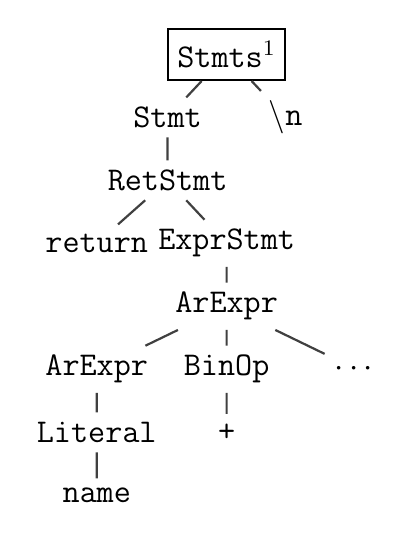
\begin{tikzpicture}
        [font=\large, edge from parent,
        % every node/.style={top color=white, bottom color=black!20,
        % ellipse, minimum size=8mm, draw=black!75,
        % thick, drop shadow, align=center},
        edge from parent/.style={draw=black!75, thick},
        level distance=0.8cm, xscale=1.0]
        \node [style={minimum size=6.5mm, draw=black, thick}] (stmts2) {\texttt{Stmts$^1$}}
        child {
            node (stmt2) {\texttt{Stmt}}
            child {
                node (RetStmt) {\texttt{RetStmt}}
                child [xscale=1.2] {
                    node (return) {\texttt{\bfseries return}}
                    }
                    child {
                        node (expr2) {\texttt{ExprStmt}}
                        child [xscale=1.1] {
                            node (arexpr1) {\texttt{ArExpr}}
                            child {
                                node (arexpr2) {\texttt{ArExpr}}
                                child {
                                    node (literal) {\texttt{Literal}}
                                    child {
                                        node (name3) {\texttt{name}}
                                    }
                                }
                            }
                            child {
                                node (binop) {\texttt{BinOp}}
                                child {
                                    node (plus) {\texttt{\bfseries +}}
                                }
                            }
                            child {
                                node (empty) {\texttt{$\cdots$}}
                            }
                        }
                    }
            }
        }
        child {
            node (newline3) {\texttt{\textbackslash n}}
        };
        \end{tikzpicture}
        }
        \subcaption{The partial parse tree generated for the example at
        \autoref{fig:bad-prog}.}
        \label{fig:partial-parse-tree-2}
    \end{minipage}
    \begin{minipage}[t]{0.31\linewidth}
        \centering
        \resizebox{\linewidth}{!}{
            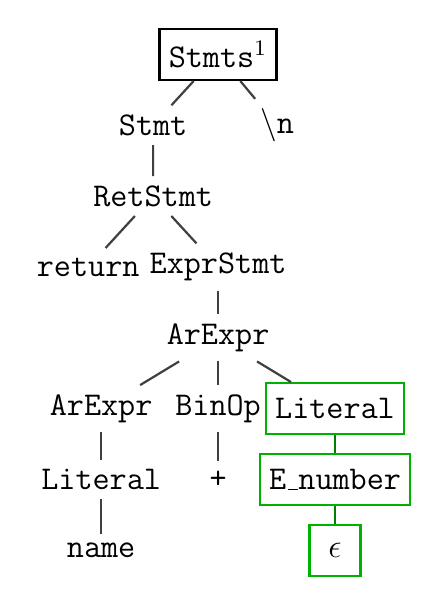
\begin{tikzpicture}
            [font=\large, edge from parent,
            % every node/.style={top color=white, bottom color=black!20,
            % ellipse, minimum size=8mm, draw=black!75,
            % thick, drop shadow, align=center},
            edge from parent/.style={draw=black!75, thick},
            level distance=0.9cm, xscale=1.0]
            \node [style={minimum size=6.5mm, draw=black, thick}] (stmts2) {\texttt{Stmts$^1$}}
            child [xscale=1.1] {
                node (stmt2) {\texttt{Stmt}}
                child {
                    node (RetStmt) {\texttt{RetStmt}}
                    child {
                        node (return) {\texttt{\bfseries return}}
                        }
                        child {
                            node (expr2) {\texttt{ExprStmt}}
                            child [xscale=0.9] {
                                node (arexpr1) {\texttt{ArExpr}}
                                child {
                                    node (arexpr2) {\texttt{ArExpr}}
                                    child {
                                        node (literal1) {\texttt{Literal}}
                                        child {
                                            node (name3) {\texttt{name}}
                                        }
                                    }
                                }
                                child {
                                    node (binop) {\texttt{BinOp}}
                                    child {
                                        node (plus) {\texttt{\bfseries +}}
                                        }
                                }
                                child {
                                    node [style={minimum size=6.5mm, draw=black!30!green, thick}] (literal2) {\texttt{Literal}}
                                    child [edge from parent/.style={draw=black!50!green, thick}] {
                                        node [style={minimum size=6.5mm, draw=black!30!green, thick}] (enumber) {\texttt{E\_number}}
                                        child {
                                            node [style={minimum size=6.5mm, draw=black!30!green, thick}] (eps) {\texttt{$\epsilon$}}
                                        }
                                    }
                                }
                            }
                        }
                }
            }
            child {
                node (newline3) {\texttt{\textbackslash n}}
            };
            \end{tikzpicture}
        } \subcaption{Adding a number with the green \texttt{E\_number} error rule.}
        \label{fig:adding-partial}
    \end{minipage}
    \begin{minipage}[t]{0.34\linewidth}
        \centering
        \resizebox{1.1\linewidth}{!}{
            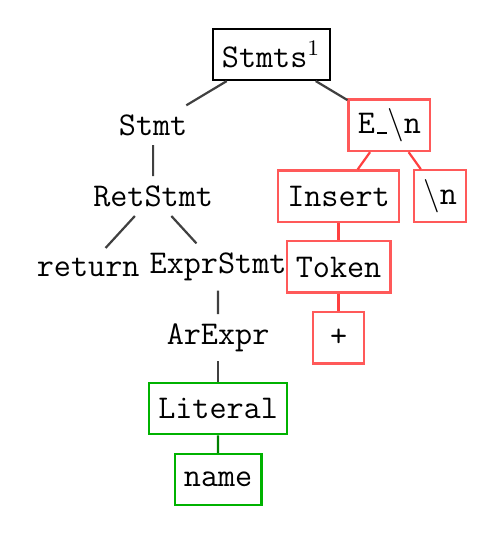
\begin{tikzpicture}
            [font=\large, edge from parent,
            % every node/.style={top color=white, bottom color=black!20,
            % ellipse, minimum size=8mm, draw=black!75,
            % thick, drop shadow, align=center},
            edge from parent/.style={draw=black!75, thick},
            level distance=0.9cm, xscale=2.0]
            \node [style={minimum size=6.5mm, draw=black, thick}] (stmts2) {\texttt{Stmts$^1$}}
            child {
                node (stmt2) {\texttt{Stmt}}
                child [xscale=0.55] {
                    node (RetStmt) {\texttt{RetStmt}}
                    child {
                        node (return) {\texttt{\bfseries return}}
                        }
                        child {
                            node (expr2) {\texttt{ExprStmt}}
                            child {
                            node (arexpr1) {\texttt{ArExpr}}
                                child {
                                    node [style={minimum size=6.5mm, draw=black!30!green, thick}] (literal1) {\texttt{Literal}}
                                    child [edge from parent/.style={draw=black!50!green, thick}] {
                                        node [style={minimum size=6.5mm, draw=black!30!green, thick}] (name3) {\texttt{name}}
                                    }
                                }
                            }
                        }
                }
            }
            child {
                node [style={minimum size=6.5mm, draw=red!65, thick}] (enewline) {\texttt{E\_\textbackslash n}}
                child [edge from parent/.style={draw=red!75, thick}, xscale=0.43] {
                    node [style={minimum size=6.5mm, draw=red!65, thick}] (insert) {\texttt{Insert}}
                    child {
                        node [style={minimum size=6.5mm, draw=red!65, thick}] (token) {\texttt{Token}}
                        child {
                            node [style={minimum size=6.5mm, draw=red!65, thick}] (plus) {\texttt{\bfseries +}}
                        }
                    }
                }
                child [edge from parent/.style={draw=red!75, thick}, xscale=0.43] {
                    node [style={minimum size=6.5mm, draw=red!65, thick}] (newline3) {\texttt{\textbackslash n}}
                }
            };
            \end{tikzpicture}
        }
        \subcaption{Deleting the \texttt{+} with red \texttt{E\_\textbackslash n} error rule.}
        \label{fig:deleting-partial}
    \end{minipage}
    \caption{The rest of the problematic function in
    \autoref{fig:partial-parse-tree-1} and two possible error correcting parses}
    \label{fig:two-partial-parses}
\end{figure}




% This eliminates backtracking and prevents a combinatorial explosion. Worst case,
% it has a time complexity of $O(n^3 G^2)$ for generic context-free grammars,
% where $n$ is the number of \emph{tokens} of the input program and $G$ is the
% grammar size, \ie the number of \emph{production rules} it includes. However,
% this parsing algorithm has limited use in large real-world programming
% languages, \eg Python or Java, and more time- and memory-efficient parsing
% algorithms are used, \eg LR parsing \etc \citep{Knuth_1965, Chapman_1987}.

% Therefore, the new and larger error correcting grammar $G'$ is introduced that
% is at least 3 times larger than $G$, making ECE-Parser not scalable for large
% programs or programs with a lot of parse errors.

However, ECE-Parser is an effective approach on finding minimum distance parses for
programs than don't belong into the given programming language, \ie have parse
errors. A straight-forward approach to keep ECE-Parser tractable is to only add a
small set of error production rules, \ie keep the size of $G'$ limited and
slightly larger than the original grammar $G$.

\subsection{Abstracting program token sequences}
\label{sec:overview:abstraction}

We need to work on programs that have parse errors, \ie we can not generate a
parse tree for them to perform all kinds of analyses that have been used in
previous work on automated program repair \citep{Sakkas_2020,
Martinez_2013,Gulwani_2018, Wang_2018} and program analysis in general.
%
The highest form of abstraction that we can use is the output of the
\emph{lexer}. The lexer tokenizes the program and returns a program \emph{token
sequence} with minimal abstractions, \eg no variable names, defining the
underlying statement blocks \etc, as shown in \autoref{fig:fixed-prog}. This
token sequence is appropriate for training our sequence classifier models, but
as we will show later on, they can contain a lot of irrelevant context for the
parse error at hand and can lead to very large sequences for our models.

\mypara{Solution: Abstract with partial parses} A \emph{parser} will hold some
internal state of the partial parses it has generated until a parse error is
encountered. The parser will then fail and return an error pointing to the
location that lead to that parse error. However, these partial parses provide
useful information and abstraction for the program at hand. For example, the
partial parse tree shown in \autoref{fig:partial-parse-tree} can be generated by
an Earley parser for the running example program. Using this partial parse tree
we can extract the \emph{abstracted token sequence} shown in the bottom of
\autoref{fig:fixed-prog}. Any \emph{completed} production rules, \eg the
one for \texttt{Params}, can be used to replace the relevant non-terminals,
\eg the parenthesis with the function arguments in this example, with the
high-level non-terminal.

\begin{figure}[t]
\centering
\begin{minipage}[c]{0.54\linewidth}
\begin{ecode}
def name ( name ) : \n
indent return name + number \n
dedent \n

def name ( name ) : \n
indent name = name + number \n
return name + \n
dedent end_marker
\end{ecode}
\subcaption{The token sequence generated by the lexer for the program.}
\label{fig:prog-seq}
\end{minipage}%
\hspace{0.02\linewidth}%
\begin{minipage}[c]{0.44\linewidth}
\begin{ecode}
FuncDef \n

def name Params : \n
indent Stmt \n
return Expr BinOp \n
dedent end_marker
\end{ecode}
\subcaption{The abstracted token sequence for the same program.}
\label{fig:abstract-prog-seq}
\end{minipage}
\caption{A simple Python program example}
\end{figure}

\mypara{Probabilistic Context-Free Grammars} Even if the original grammar $G$ is
not ambiguous, generating partial parses can be ambiguous. Earley parsing is an
dynamic programming technique and internally keeps all possible parses from the
begging of the token sequence until a position $i$ in its charts. Therefore,
when there is a parse error at token $i$, it is possible to have more than one
partial parses to choose from in order to generate the abstracted token
sequence. For the running example, if we focus on the \texttt{return} statement
of the program, there are two possible partial parses in the parser chart, as
shown in \autoref{fig:two-partial-parses} for example, that we can use to repair
the program. \autoref{fig:adding-partial} would lead to a solution that
completes the returned arithmetic expression by adding the blue node, which is
another arithmetic expression and possibly just another number, while the
\autoref{fig:deleting-partial} would produce a solution that returns just the
number by deleting the arithmetic operator in the red node.

In that aid, Probabilistic Context-Free Grammars (PCFGs) have been used in
previous work \citep{Collins_2013, Jelinek_1992} to select \emph{complete}
parses for ambiguous grammars. A PCFG associates each of its production rules
with a \emph{weight} or \emph{probability}. Each parse tree that is generated
during parsing is also associated with a probability. Finally, the one with the
highest probability is selected as a final parse tree. A PCFG can simply be
learned \citep{Collins_2013} by counting the production rules used to parse a
number of programs belonging to that language for each terminal token.

We apply this approach to select a partial parse from the Earley parser. The
probabilities can again be learned from the \emph{fixed} programs of a large
corpus of erroneous and fixed programs. The selected partial parse can then be
used to generate an abstracted token sequence.


\subsection{Training Sequence Classifiers}
\label{sec:overview:train}
The abstracted token sequences we extracted from the partial parses present us
with shorter abstracted sequences that maintain a lot of the program's context
along with some hints of the user's intended behavior for the program due to the
PCFG usage. Additionally, recent work on machine learning, and especially on
Natural Language Processing (NLP) \citep{Sutskever_2014, Hardalov_2018}, have
utilized \emph{sequence models} to learn underlying patterns in their data.
These models stand out in domains where the input is a sequence and feature
extraction methods are not readily available to utilize in order to use the
older classic neural network models \citep{Sutskever_2014}.

\mypara{Sequence models} Sequence-to-sequence (seq2seq) architectures aim to
transform a input sequence of tokens into a new sequence \citep{Sutskever_2014}.
These architectures consist of an \emph{encoder} and a \emph{decoder}. The
encoder transforms the input token sequence into a \emph{$n$-dimensional
abstract vector} that captures all the essence and context of the input
sequence. This vector doesn't necessarily have some physical meaning and is just
an internal representation of the input sequence into a higher dimensional
space. The abstract vector is given as an input to the decoder, which in turn
transforms it into a output sequence. Both the encoder and the decoder can be an
(older) Long-Short-Term-Memory (LSTM)-based model \citep{Hochreiter_1997} or a
state-of-the-art \emph{Transformer} \citep{Vaswani_2017}.

\mypara{Transformer Classifier} We desire to train a model that can correctly
predict a small set of error production rules for a given abstracted token
sequence. We encode this problem into a \emph{supervised multi-class
classification}. A \emph{supervised} learning problem is one where, given a
labeled training set, the task is to learn a function that accurately maps the
inputs to output labels and generalizes to future inputs. In a
\emph{classification} problem, the function we are trying to learn maps inputs
to a discrete set of two or more output labels, called \emph{classes}.
Therefore, we encode the task of learning a function that will map token
sequences of erroneous programs to a small set of error production rules as a
\emph{multi-class} classification (MCC) problem. We use an \emph{encoder
transformer} to encode the input sequences into abstract vectors that we can
then feed into a \emph{Deep Neural Network (DNN)} classifier to train it and
make predictions.

\mypara{Predicting Error Rules via MCC}
Given a dataset of fixed parse errors, we can extract the small set of error
rules needed for each program to make it parse with an ECE-Parser. Running ECE-Parser on
every program in the dataset is prohibitively slow. Therefore, we extract the
erroneous and fixed program token-level differences or \emph{token diffs} and
map them to error production rules. After this prodecure, we run ECE-Parser with the
learned error rules to confirm which ones would make the program parse and
assign them as \emph{labels}.

We then train a Transformer classifier on a new updated error-rule-labeled data
set. Futhermore, Neural networks have the advantage of associating each class
with a \emph{confidence score} that can be interpreted as the model's confidence
of each class being correct for a given input. Therefore, confidence scores can
be used to rank error rule predictions for new programs and select the top-$N$
ones that will maintain a decent performance when used with the ECE-Parser. Exploiting
recent advances in machine learning, we use deep and dense architectures
\citep{Schmidhuber_2015} for more accurate predictions.

\section{Abstracting Programs with Parse Errors}
\label{sec:prog-abstract}

\mypara{Program Lexer}

\mypara{Token Sequences}


\subsection{Earley Partial Parses} \label{sec:prog-abstract:partial}

\mypara{Problem: Multiple Partial Parses}

\mypara{Example}


\subsection{Probabilistic Context-Free Grammars}
\label{sec:prog-abstract:pcfg}

\mypara{Constructing a PCFG}

\mypara{Example of PCFG}

\mypara{Example}

\subsection{From Programs to Abstract Token Sequences}

\mypara{Explain Pseudocode combining PCFG + Most Likely}

\mypara{Example: Selecting Most Likely Partial Parse}




\section{Training Sequence Classifiers}
\label{sec:seq-classifiers}

Our next task is to \emph{train} a model that can predict the error production
rules that are needed to parse a given program $e_{\bot}$ (with syntax errors)
according to a given grammar $G$, by using its (abstracted) program token
sequence $t^a$.
%
We define the function $\predictDLsym$ which takes as input a \emph{pre-trained
sequence classifier} $\Model$ and an abstracted token sequence $t^a$ and returns
as output a \emph{small subset} of $\errorrulessym$.
%
We train the $\Model$ offline with the $\trainDLsym$ method with a dataset
$\List{t^a \times \errorrulessym}$ of token sequences $t^a$ and the \emph{exact
small set} of error production rules $\errorrulessym$ that the ECE-Parser used
to generate the \emph{user parse}. We build our classifier $\Model$ using
classic \emph{Deep Neural Networks (\dnn{}s)} and parts of state-of-the-art
\emph{Sequence-to-Sequence (seq2seq)} models. We leave the high level details of
acquiring the dataset of labeled token sequences and using the predictor for new
erroneous programs for \autoref{sec:whole-system}. In the next few paragraphs,
we summarize the recent advances in machine learning that help as build the
sequence classifier.

We encode the task of learning a function that will map token sequences of
erroneous programs to a small set of error production rules as a
\emph{supervised multi-class classification (MCC)} problem. A \emph{supervised}
learning problem is one where, given a labeled training set, the task is to
learn a function that accurately maps the inputs to output labels and
generalizes to future inputs. In a \emph{classification} problem, the function
we are trying to learn maps inputs to a discrete set of two or more output
labels, called \emph{classes}. We use a \emph{Transformer encoder} to encode the
input sequences into abstract vectors that we then directly feed into a
\emph{\dnn} classifier to build a \emph{Transformer classifier}.

\mypara{Neural Networks}
A neural network can be represented as a directed acyclic graph whose nodes are
arranged in layers that are fully connected by weighted edges. The first layer
corresponds to the input features, and the final to the output. The output of an
internal node is the sum of the weighted outputs of the previous layer passed to
a non-linear \emph{activation function}, which in recent work is commonly chosen
to be the rectified linear unit (ReLU) \citep{Nair2010-xg}. In this work, we use
relatively \emph{deep neural networks} (\dnn) that have proven to make more
accurate predictions in recent work~\citep{Schmidhuber_2015}. A thorough
introduction to neural networks is beyond the scope of this
work~\citep{Hastie2009-bn, Nielsen2015-pu}.

% For example, the outputs of an internal layer of nodes $l$ is given as $y_l =
% g(W_{l-1} y_{l-1})$, where $W_{l-1}$ is the weight matrix for the edges between
% layers $l$ and $l-1$ and $y_{l-1}$ is the output of the previous layer. The
% input $y_0 = x$ is the input features of the neural network and, finally, g is
% the activation function, which in recent work is commonly chosen to be the
% rectified linear unit (ReLU), defined as $g(x) = max(0, x)$ \citep{Nair2010-xg}.
% The number of layers, the number of nodes per layer, and the connections between
% layers constitute the \emph{architecture} of a neural network

\mypara{Sequence Models}
\emph{Seq2seq} models aim to transform input sequences of one domain into
sequences of another domain \citep{Sutskever_2014}. In the general case, these
models consist of two major layers, an \emph{encoder} and a \emph{decoder}. The
encoder transforms an input token sequence $x_1, x_2, \dots, x_n$ into a
\emph{abstract vector} $V \in \R^k$ that captures all the essence and context of
the input sequence. This vector does not necessarily have some physical meaning
and is just an internal representation of the input sequence into a higher
dimensional space. The abstract vector is then given as an input to the decoder,
which in turn transforms it into an output sequence $y_1, y_2, \dots, y_n$.

% \begin{align}
%     h_t &= f(W_{hx} x_t + W_{hh} h_{t-1}) \label{eq:1} \\
%     y_t &= g(W_{yh} h_t) \label{eq:2}
% \end{align}

The simplest approach historically uses a Recurrent Neural Network (RNN)
\citep{Rumelhart1986, Werbos1990}, which is a natural next step from the classic
neural networks. Each RNN unit operates on each input token $x_t$ separately. It
keeps an internal \emph{hidden state} $h_t$ that is calculated as
% in $h_t = f(W_{hx} x_t + W_{hh} h_{t-1})$,
a function of the input token $x_t$ and the previous hidden state $h_{t-1}$.
% The weight matrices $W_{hx}$ and $W_{hh}$ parametrize the input-to-hidden and
% the hidden-to-hidden connections respectively. The function $f$ is another
% non-linear activation function such as \emph{tanh, sigmoid} and \emph{ReLU}.
The output $y_t$ is calculated as
% $y_t = g(W_{yh} h_t)$, \ie
the product of the current hidden state $h_t$ and an output weight matrix. The
activation function is usually chosen as the standard \emph{softmax} function
\citep{Goodfellow-et-al-2016, Bishop-book-2006}. Softmax assigns probabilities
to each output that must add up to 1.
% which, for an output vector $y = (y_1, \dots, y_N) \in \R^{N}$, is defined as:
% \[ \sigma(y)_i = \frac{e^{y_i}}{\sum_{j=1}^{N} e^{y_j}},\ for\ i = 1, \dots, N.
% \]
Finally, the loss function at all steps of the RNN is typically calculated as
the sum of the cross-entropy loss of each step.

% These recurrent models have to generate the sequence of hidden states $h_t$, as
% a function of the previous hidden state $h_{t-1}$ and the input $x_t$. This
% sequential generation of hidden states limits parallelization within training
% examples and causes training problems when dealing with longer sequences, as
% memory constraints limit batching across examples. However, the latest
% state-of-the-art approach for seq2seq architectures is the newer
% \emph{Transformer} model \citep{Vaswani_2017} that replaces the classic RNN unit
% and solves these problems due to its \emph{attention mechanisms}.

\mypara{Transformers}
The Transformer is an \dnn architecture that deviates from the recurrent pattern
(\eg, RNNs) and is solely relying on \emph{attention mechanisms}. Attention has
been of interest lately \citep{Bahdanau2015, Kim2017, Vaswani_2017} mainly due
to its ability to detect dependencies in the input or output sequences
regardless the distance of the tokens. The nature of this architecture makes the
Transformer significantly easier to parallelize and thus has a higher
quality of predictions and sequence translations after a shorter training
period.

The novel architecture of a Transformer \citep{Vaswani_2017} is structured as a
\emph{stack of $N$ identical layers}. Each layer has two main sub-layers. The
first is a \emph{multi-head self-attention mechanism}, and the second is a
position-wise fully connected neural network. The output of each sub-layer is
$LayerNorm(x + SubLayer(x))$, where $SubLayer(x)$ is the function implemented by
each sub-layer, followed by a residual connection around each of the two
sub-layers and  by layer normalization $LayerNorm(x)$. To facilitate these
residual connections, all sub-layers in the model, as well as the input
\emph{embedding layers}, produce outputs of the same dimension $d_{model}$.

% This architecture is used as described above in a seq2seq model
% \citep{Vaswani_2017} for the encoder. The decoder would require an extra third
% sub-layer, which performs multi-head attention over the output of the encoder
% stack. However, in our task we learn sets of error production rules, which we
% frame as a classic \emph{multi-class classification} problem. We are dealing
% with input sequences of varied sizes, where no straightforward feature
% extraction technique exists. Therefore, we utilize the effectiveness of the
% state-of-the-art \emph{Transformer encoder} to summarize the programs into
% fixed-length vectors that can then be fed into classic \dnn{} classifiers.

% \subsection{Transformer Classifier}
% \label{sec:seq-classifiers:location-rank}


% \mypara{Multi-class \dnn{}s}
%
% A \dnn can be used as a binary classifier, \ie predict if the given input
% belongs into a class or not. While this model is enough for many tasks, \eg
% error localization \citep{Sakkas_2020, Seidel:2017}, in the case of error rule
% prediction we have to select from multiple \emph{classes}. We therefore use a
% \dnn for our error rule prediction $\Model$, but we adjust the output layer to
% have $N$ nodes for the selected $N$ error-rule-classes.

% \mypara{Multi-class Transformer Classifiers}
%
\mypara{Transformer Classifier}
For our task, we choose to structure $\Model$ as a \emph{Transformer
Classifier}. We use a novel Transformer encoder to represent an abstracted token
sequence $t^a$ into an abstract vector $V \in \R^k$. The abstract vector $V$ is
then fed as input into a multi-class \dnn. We use $\trainDLsym$ to train the
$\Model$ given the training set $\List{t^a \times \errorrulessym}$. The binary
cross-entropy loss function is used per class to assign the loss per training
cycle. $\Model$ predicts error production rules for a new input program $t^a$.
Critically, we require that the classifier outputs \emph{confidence scores}
$\Conf$ that measure how sure the classifier is that a rule can be used to parse
the associated input program $e_{\bot}$. The $\predictDLsym$ function uses the
trained $\Model$ to predict the confidence scores $\List{\errorrulessym\ \times\
\Conf}$ for all error production rules $\errorrulessym$ for a new unknown
program $e_\bot$ with syntax errors. The $\errorrulessym$ are then sorted based
on their predicted confidence score $\Conf$ and finally the \emph{top-N} rules
are returned for error-correcting parsing. $N$ is a small number in the 10s that
will give accurate predictions without making the ECE-Parser too slow, as we
discuss in \autoref{sec:eval}.

\section{Building a Fast Error-Correcting Parser}
\label{sec:whole-system}

We show how $\systemsym$ uses the abstracted token sequences from
\autoref{sec:prog-abstract} and the trained sequence models from
\autoref{sec:seq-classifiers} to generate an \emph{error-correcting parser}
$(e_{\bot} \to e)$, that will parse an input program $e_{\bot}$ with syntax
errors and produce a correct program $e$. We first describe how we extract a
machine-learning-amenable training set from a corpus of fixed programs and
finally how we structure everything to train our model.


\subsection{Learning Error Production Rules}
\label{sec:whole-system:error-rules}

The $\trainDLsym$ method requires a dataset of token sequences $t^a$ that is
annotated with an \emph{exact and small set} of error production rules, \ie
$\List{t^a \times \errorrulessym}$. These $\errorrulessym$ are just a subset of
all the possible error rules that are needed to parse and fix $t^a$. The
straight-forward approach is to use $\ecepsym$ with all possible error
production rules for each program $e_{\bot}$ in the dataset. Then, when
$\ecepsym$ returns with a successful parse, we extract the rules that where used
to parse the program $e_{\bot}$. This approach generates a dataset with the
smallest possible set of error rules as labels per program, since the original
ECE-Parser returns the minimum-distance edit parse. However, this approach
completely ignores the programmer's fix and takes an unreasonable amount of time
to parse a dataset with millions of programs, due to the inefficient nature of
the ECE-Parser.

We suggest using an $O(ND)$ difference algorithm \citep{Myers_1986} to get a
small but still representative set of error production rules for each program
$e_{\bot}$. We employ this algorithm to find the differences between the input
\emph{program token sequence} $t^i$, which is the lexed program $e_{\bot}$ and
the \emph{fixed token sequence} $t^o$, which is the lexed program $e$. This
algorithm returns changes between token sequences in the form of \emph{inserted
or deleted tokens}. It is possible that this algorithm returns a sequence of
deletions followed by a sequence of insertions, which can in turn be interpreted
as a \emph{replacement} of tokens. We map these three types of changes to the
respective error production rules. Let $t^i$ be a sequence $t^i_1, t^i_2, \dots,
t^i_n$ and $t^o$ be the updated sequence $t^o_1, t^o_2, \dots, t^o_m$. We map:
\begin{itemize}
    \item an inserted output token $t^o_j$ to a \emph{deletion} error $E_{t^o_j}
    \rightarrow \epsilon$.
    \item a deleted input token $t^i_k$ to an \emph{insertion} error $Tok\
    \rightarrow t^i_k$ and the helper rule $E_{t^i_{k+1}} \rightarrow Ins\
    t^i_{k+1}$.
    \item a replaced token $t^i_k$ with $t^o_j$ to a \emph{replacement} error
    $Repl\ \rightarrow t^i_k$ and the helper rule $E_{t^o_j} \rightarrow Repl$.
\end{itemize}

In the case of an insertion error, we also include the helper rules $Ins\
\rightarrow\ Tok$ and $Ins\ \rightarrow\ Ins\ Tok$, that can derive any nonempty
sequence of insertions. To introduce (possible) insertion errors at the end of a
program, we include the starting production rules $S' \rightarrow S$ and $S'
\rightarrow S\ Ins$.

The above algorithm, so far, adds only the \emph{terminal error productions}. We
have to include the \emph{non-terminal error productions} that will invoke the
terminal ones. If $X \rightarrow a_0b_0a_1b_1 \dots a_mb_m,\ m \geq 0$, is a
production in $P$ such that $a_i$ is in $N^*$ and $b_i$ is in $\Sigma$, then we
add the error production $X \rightarrow a_0X_{b_0}a_1X_{b_1} \dots a_mX_{b_m},\
m \geq 0$ to $P'$, where each $X_{b_i}$, is either a new non-terminal $E_{b_i}$
that was added with the previous algorithm, or just $b_i$ again if it was not
added.

Finally, we further refine the new small set of error productions for each
program $e_{\bot}$ with ECE-Parser, in order to create the final annotated
dataset $\List{t^a \times \errorrulessym}$. The changes that we extracted from
the programmers' fixes might include irrelevant changes to the parse error fix,
\eg code clean-up. Therefore, filtering with the ECE-Parser is still essential
to annotate each program with the appropriate error production rules. We
implement this error-rule-extracting approach in the function $\diffsym$, which
extracts the token differences between an erroneous program $e_{\bot}$ and a
fixed program $e$ and returns the appropriate error production rules.


\subsection{Training and Using a Transformer Classifier}
\label{sec:whole-system:training-classifier}

\begin{figure}[t]
  \centering
  \begin{minipage}[t]{0.49\linewidth}
    \centering
    \begin{algorithm}[H]
    \caption{Training $\systemsym$'s model $\Model$}
    \label{algo:training-classifier-algo}
    \renewcommand{\algorithmicrequire}{\textbf{Input:}}
    \renewcommand{\algorithmicensure}{\textbf{Output:}}
    \begin{algorithmic}[1]
    \Require{Probabilistic Grammar $G$, $\datasetsym\ Ds$}
    \Ensure{Classifier $Model$}
    \Procedure{Train}{$G,\,Ds$}
    \State $D_{ML} \gets \emptyset$
    \ForAll{$\pbad \times \pfix \in Ds$}
      \State $t^a \gets$ \Call{PartialParse}{$G,\,\pbad$}
      \State $rules \gets$ \Call{DiffRules}{$\pbad \times \pfix$}
      \State $D_{ML} \gets D_{ML}\,\cup\ (t_a \times rules)$
    \EndFor
    \State $Model \gets$ \Call{TrainDL}{$D_{ML}$}
    \State \Return{$Model$}
    \EndProcedure
    \end{algorithmic}
\end{algorithm}

  \end{minipage}
  \hspace{0.02\linewidth}
  \begin{minipage}[t]{0.47\linewidth}
    \centering
    \begin{algorithm}[H]
    \captionsetup{font=small}
    \caption{Predicting error production rules with $\systemsym$'s model $\Model$}
    \label{algo:predict-algo}
    \renewcommand{\algorithmicrequire}{\textbf{Input:}}
    \renewcommand{\algorithmicensure}{\textbf{Output:}}
    \begin{algorithmic}[1]
    \Require{Classifier $Model$, Probabilistic Grammar $G$, Program $P$}
    \Ensure{Error Production Rules $Rls$}
    \Procedure{Predict}{$Model,\,G,\,P$}
    \State $t^a \gets$ \Call{PartialParse}{$G,\,P$}
    \State $Rls \gets$ \Call{PredictDL}{$Model,\,t^a$}
    \State \Return{$Rls$}
    \EndProcedure
    \end{algorithmic}
\end{algorithm}

  \end{minipage}
\end{figure}

% \mypara{Training the Transformer Classifier}
%
Given a (probabilistic) grammar $G$ and a dataset $Ds$,
\Cref{algo:training-classifier-algo} extracts a machine-learning appropriate
dataset $D_{ML}$ in order to $\trainsym$ a Transformer classifier $Model$ with
$\trainDLsym$. The classifier $Model$ can then be used to predict error rules
for new erroneous programs $\pbad$.

The dataset $D_{ML}$ starts as an empty set. For each program pair $\pbad \times
\pfix$, we, first, employ $\partialsym$ with the PCFG $G$ and an erroneous
program $\pbad$ to extract the abstracted token sequence $t^a$. Second, we use
the token difference algorithm $\diffsym$ to extract the specific error $rules$
that fix $\pbad$ based on $\pfix$. The abstracted sequence $t^a$ is annotated
with the label $rules$ and is added to $D_{ML}$. The Transformer classifier
$Model$ is trained with $\trainDLsym$ and the newly extracted dataset $D_{ML}$,
which is finally returned by the algorithm. Finally, the $\trainsym$ing
procedure can be performed offline and thus won't affect the performance of the
final program repair.

% \mypara{Predicting Error Rules}
%
Having trained the Transformer classifier $Model$, we can now predict error
rules $Rls$, that will be used by an ECE-Parser, by using the $\predictsym$
procedure defined in \Cref{algo:predict-algo}. $\predictsym$ uses the same input
grammar $G$ to generate an abstracted token sequence $t^a$ for the program $P$
with the $\partialsym$ procedure. Finally, the $\predictDLsym$ procedure
predicts a small set of error production rules $Rls$ for the sequence $t^a$
given the pre-trained $Model$.

\subsection{Generating an Efficient Error-Correcting Parser}
\label{sec:whole-system:building-ecp}

\begin{algorithm}[t]
    \caption{Generating the final ECEP}
    \label{algo:ecep-algo}
    \renewcommand{\algorithmicrequire}{\textbf{Input:}}
    \renewcommand{\algorithmicensure}{\textbf{Output:}}
    \begin{algorithmic}[1]
    \Require{Grammar $G$, $\datasetsym\ Ds$}
    \Ensure{Error Correcting Parser $Prs$}
    \Procedure{Seq2Parse}{$G,\,Ds$}
    \State $Model \gets$ \Call{Train}{$G,\,Ds$}
    \State \textsc{ERulePredictor} $\gets$ \Call{Predict}{$Model$}
    \State $Prs \gets (\lambda.\pbad \to$ \Call{EarleyECParse}{\Call{ERulePredictor}{$\pbad$}$,\,\pbad$}$)$
    \State \Return{$Prs$}
    \EndProcedure
    \end{algorithmic}
\end{algorithm}


\Cref{algo:ecep-algo} presents our \emph{neurosymbolic} approach, $\systemsym$.
This is the high-level algorithm that combines everything that we described so
far in the last three sections. $\systemsym$ first extracts the fixed programs
$ps$ from the dataset $Ds$ to learn a probabilistic context-free grammar $PCFG$
for the input grammar $G$ with $\learnPCFGsym$. It then $\trainsym$s the
Transformer classifier $Model$ to predict error production rules. We define an
error rule predictor, \textsc{ERulePredictor}, using the $\predictsym$ procedure
with the pre-trained $Model$ and grammar $PCFG$. Finally, the algorithm returns
the ECE-Parser $Prs$, which we define as a function that takes as input an
erroneous program $\pbad$ that uses the \textsc{ERulePredictor} to get the set
of error rules needed by $\ecepsym$ to parse and repair it.

\section{Evaluation}
\label{sec:eval}

We have implemented our approach in \toolname: a system for repairing parse
errors for \python at its entirety. Next, we describe our implementation and an
evaluation that addresses four questions:

\begin{itemize}
    \item \textbf{RQ1}: How \emph{accurate} are \toolname's predicted error production rules?
                        (\S~\ref{sec:eval:accuracy})
    \item \textbf{RQ2}: How \emph{precisely} can \toolname repair parse errors?
                        (\S~\ref{sec:eval:precise})
    \item \textbf{RQ3}: How \emph{efficiently} can \toolname repair parse errors?
                        (\S~\ref{sec:eval:efficiency})
    \item \textbf{RQ4}: How \emph{useful} are \toolname's suggested repairs?
                        (\S~\ref{sec:eval:useful})
\end{itemize}

% \subsection{Implementation} \label{sec:eval:gen_method}

\mypara{Training Dataset}
For our evaluation, we use the \python dataset we used in our error data
analysis in \autoref{sec:error-analysis} gathered from
PythonTutor.com~\citep{Guo2013} between the years 2017 and 2018. The dataset has
more than 1,100,000 usable erroneous Python programs and their respective fixes.
The programs have an average length of \emph{87 tokens}, while the abstracted
token sequences have a much shorter average of \emph{43 tokens}. We use 15,000
random programs from the dataset for all our tests, and the rest we use as our
training set.

We first learn a PCFG on the training set of fixed programs in order to learn
the probabilities for each production rule in the \emph{full set of the \python
grammar}. \toolname then extracts the abstracted token sequences for all
programs in the training set. Next, while for the full set of \python there are
\emph{455 possible terminal error production rules} that \toolname's can predict
from, in reality only \emph{340 error rules} are ever used in the full dataset.
We arrive at this set of error rules by parsing all the erroneous programs in
the training set with the ECE-Parser and the "diff" error rules, as described in
\autoref{sec:overview:train}. Each program is also assigned as labels these
error rules that make the ECE-Parser parse the erroneous program successfully.

\mypara{Transformer Classifier}
\toolname's error rule prediction uses a Transformer classifier with \emph{six}
transformer blocks, that each has a fully-connected hidden layer of 256 neurons
and 12 attention heads. The output of the transformer blocks is then connected
to a \dnn based classifier with \emph{two} fully-connected hidden layers of 256
and 128 neurons respectively. The neurons use rectified linear units (ReLU) as
their activation function \citep{Nair2010-xg}, while the output layer uses the
sigmoid function for each class \citep{Nielsen2015-pu}. Additionally, the are
\emph{two input embedding layers} of a length of 128, one for input tokens and
one for their positions in the sequence. We also limit the size of the input
abstracted token sequences to a length of 128, which covers $95.7\%$ of the
training set, without the need of pruning them. Finally, the Transformer
classifier was trained using an \textsc{Adam} optimizer \citep{Kingma2014-ng}, a
variant of stochastic gradient descent that converges faster, for a total of 50
epochs.

\subsection{RQ1: Accuracy}
\label{sec:eval:accuracy}

We consider \toolname's transformer classifiers' accuracy up to the \emph{top
50} error production rules predictions against our original and the final
version of our approach

% colors from http://colorbrewer2.org/?type=sequential&scheme=Blues&n=3
\definecolor{blue1}{HTML}{DEEBF7}
\definecolor{blue2}{HTML}{9ECAE1}
\definecolor{blue3}{HTML}{3182BD}
\definecolor{green1}{HTML}{E5F5E0}
\definecolor{green2}{HTML}{A1D99B}
\definecolor{green3}{HTML}{31A354}

\begin{figure}[t]
  % \begin{minipage}[c]{0.49\linewidth}
    \centering
    \resizebox{!}{0.25\textheight}{
      \Large
      \begin{tikzpicture}
      \begin{axis}[
        ybar stacked,
        width=1.2\linewidth,
        height=10cm,
        % title={Accuracy of Repair Template Prediction},
        ylabel={Prediction Accuracy (\%)},
        bar width=1.2cm,
        ymin=0.0,
        ymax=101.0,
        ytick={0.0, 10.0, 20.0, 30.0, 40.0, 50.0, 60.0, 70.0, 80.0, 90.0, 100.0},
        yticklabel={\pgfmathparse{\tick}\pgfmathprintnumber{\pgfmathresult}},
        ytick style={draw=none},
        ymajorgrids = true,
        symbolic x coords={original, abstracted, abstracted-best},
        enlarge x limits=0.3,
        xtick=data,
        xtick style={draw=none},
        xticklabels={\textsc{Original}\xspace, \textsc{Abstracted}\xspace, \textsc{Threshold}\xspace},
        %x tick label style={rotate=45, anchor=north east},
        x tick label style={font=\LARGE},
        y tick label style={font=\LARGE},
        label style={font=\LARGE},
        reverse legend,
        % transpose legend,
        legend style={legend pos = north east, legend columns=4, font=\large},
      ]

      \addplot[draw=black, fill=blue2, bar shift=-.601cm, postaction= { pattern=dots }] coordinates {(original, 0.0) (abstracted, 0.0) (abstracted-best, 79.28025102961365)};

      \resetstackedplots

      \addplot[draw=black, fill=green2, bar shift=.601cm, postaction= { pattern=dots }] coordinates {(original, 0.0) (abstracted, 0.0) (abstracted-best, 69.82968369829683)};

      \resetstackedplots

      \addplot[draw=black, fill=green1, bar shift=.601cm] coordinates {(original, 12.875536480686696) (abstracted, 58.394160583941606) (abstracted-best, 0.0)};
      \addlegendentry{Top-10}
      \addplot[draw=black, fill=green2, bar shift=.601cm] coordinates {(original, 20.100143061516448) (abstracted, 14.922952149229523) (abstracted-best, 0.0)};
      \addlegendentry{Top-20}
      \addplot[draw=black, fill=green3, bar shift=.601cm] coordinates {(original, 31.974248927038623) (abstracted, 15.49067315490673) (abstracted-best, 0.0)};
      \addlegendentry{Top-50}
      \addlegendimage{empty legend}
      \addlegendentry{Rare:}

      \resetstackedplots

      \addplot[draw=black, fill=blue1, bar shift=-.601cm] coordinates {(original, 56.712132089016514) (abstracted, 72.11217885859972) (abstracted-best, 0.0)};
      \addlegendentry{Top-10}
      \addplot[draw=black, fill=blue2, bar shift=-.601cm] coordinates {(original, 11.769733018835673) (abstracted, 9.335163757599531) (abstracted-best, 0.0)};
      \addlegendentry{Top-20}
      \addplot[draw=black, fill=blue3, bar shift=-.601cm] coordinates {(original, 18.65107852186101) (abstracted, 11.253840622344256) (abstracted-best, 0.0)};
      \addlegendentry{Top-50}
      \addlegendimage{empty legend}
      \addlegendentry{All:}

      \end{axis}
      \end{tikzpicture}
    }
    \caption{
      Results of our error production rule prediction classifiers for the simple original token sequences and their abstracted versions using the PCFG. \GS{TODO: Should we add here the Abstracted results without the PCFG???}
    }
    \label{fig:accuracy-results}
  % \end{minipage}
  % \begin{minipage}[c]{0.49\linewidth}
  %   \centering
  %   \includegraphics[width=\linewidth]{accuracy-per-change.pdf}
  %   \caption{The repair accuracy for the number of edits needed by the user to repair.}
  %   \label{fig:accuracies-per-changes}
  % \end{minipage}
\end{figure}


\mypara{Results: Accuracy of Error Rule Prediction}
%
\autoref{fig:accuracy-results} shows the accuracy results of our error
production rule prediction experiments. The y-axis describes the fraction of
programs for which the \emph{whole} set of the needed error rules needed to
repair the \emph{erroneous} program was a complete subset of the top-K predicted
rules.
%
The \textsc{Original} version of our transformer classifier didn't consider the
partial parses produced with the PCFG's aid and used the full \textsc{Original}
token sequences, whose results are presented in the first two bars of
\autoref{fig:accuracy-results}. The next two bars show our final results using
the \textsc{Abstracted} token sequences to train the classifier. Finally, the
last two dotted bars show the results for when a \textsc{Threshold} is set in
order to select the predicted error rules, instead of picking the static top-K
ones. The predicted error rule set can have a size anywhere between 1 and a
maximum of 25 (pre-defined by us based on the top-K results).

The blue bars show the accuracy on the full test set of \textsc{All} 15,000
programs, while the green bars show the results on the subset of \textsc{Rare}
programs, \ie the programs that didn't include any of the 50 most popular error
rules, that amount only for 4.8\% of our test set.

The \textsc{Original} predictor, even with the Top-50 predicted error rules is
less accurate than the Top-20 predictions of the \textsc{Abstracted}, with an
accuracy of 73.96\%, which drops to 51.16\% and 32.34\% respectively for the
Top-20 and Top-10 predictions. The \textsc{Abstracted} predictor significantly
outperforms the \textsc{Original} predictor with a 72.08\% Top-10 accuracy,
81.08\% Top-20 accuracy and 92.13\% Top-10 accuracy.

The \textsc{Threshold} predictions are almost as accurate as the
\textsc{Abstracted} Top-20 predictions with an accuracy of 79.46\% and a median
number of selected error rules of 12 (average 13.9). This could potentially mean
that this predictor is a valid alternative for the static Top-20 predictions.

Finally, we observe that our \textsc{Abstracted} classifiers generalize
efficiently for our dataset of erroneous \python programs and is almost as
accurate as the rest of the dataset with a 74.11\% Top-20 accuracy (85.69\%
Top-50 accuracy). The same holds for the \textsc{Threshold} predictions with a
72.46\% accuracy.

\begin{framed}
  \noindent \toolname's transformer classifier learns to encode programs with
  syntax errors and select candidate error production rules for them
  effectively, yielding \emph{high accuracies}. By abstracting the tokens
  sequences, \toolname is able to \emph{generalize} better and make more
  accurate predictions with a \emph{81.08\% Top-20 accuracy}.
\end{framed}


\subsection{RQ2: Repaired Program Preciseness}
\label{sec:eval:precise}

\begin{table}[t]
  \centering
  \begin{tabular}{l||cccc}
    Error Rule Approach            & Parse Accuracy & User Parse Rate & Parse time & Speedup \\
    \hline
    20 Most Popular                & 79.81\% & 16.31\% & 4.8 sec  & 45.8 sec \\
    50 Most Popular                & 90.03\% & 18.55\% & 10.6 sec & 37.1 sec \\
    Top-20 (\textsc{All-Parses})   & 59.31\% & 30.57\% & 15.6 sec & 57.4 sec \\
    Top-20 (\textsc{Minimum-Cost}) & 92.45\% & 19.95\% & 4.1 sec  & 68.0 sec \\
  \end{tabular}
  \caption{Experimental results of \toolname's repair approaches.}
  \label{tab:seq2parse_full_results}
\end{table}

Next we evaluate \toolname's end-to-end accuracy and preciseness in generating
valid parses for programs with syntax errors. For all of our tests we limit the
\toolname's parsing to \emph{5 mins} and run our experiments on \emph{15,000
erroneous programs} from our dataset. The rest of the dataset was used to train
our transformer classifiers, and specifically here the \textsc{Abstracted}
classifier.

We compare our \emph{two versions} of our implementation of \toolname
(\textsc{All-Parses} and \textsc{Minimum-Cost}) against two versions of the
error-correcting parser with a static selection of the 20 and 50 most popular
error production rules in our training set. We make this comparison because we
observe in our training set that the 50 most of popular error rules are used for
parsing as much as \emph{86\%} of the dataset.

Our \textsc{All-Parses} ECEP and \textsc{Minimum-Cost} ECEP both use the
\emph{Top-20 predictions} from our \textsc{Abstracted} classifier to generate
parses and thus generate full program repairs. The \textsc{All-Parses} ECEP
keeps internally all possible states that arise from using the predicted error
rules and having a maximum repair cost of 2 edits (\ie a maximum of 2
insertions, deletions or replacements). The \textsc{Minimum-Cost} version
however keeps always the minimum-edit repair and discards all other states that
may lead to a higher cost. This allows for a higher maximum cost of 10 edits.
Finally, while \textsc{All-Parses} can generate a large number of repairs, we
keep only the top 3 repairs after filtering with a static code checker
(\textsc{Pylint}, \url{https://www.pylint.org/}) as most developers will
consider at most five suggestions before falling back to manual debugging
\citep{Kochhar2016-oc, Parnin2011-ce}.

\autoref{tab:seq2parse_full_results} shows the percentage of test programs that
each of these four versions can parse successfully (\ie the parse accuracy) and
the amount of parses that match the one that user compiled. We observe that the
Top-20 predictions with the \textsc{Minimum-Cost} ECEP \emph{outperforms} every
other option in parse accuracy and parse time, with 92.45\% and 4.1 seconds
respectively. It also achieves to generate the intended parse for 19.95\% of the
set, \ie in almost 1 out 5 of the cases. The 20 most popular ECEP with 79.81\%
parse accuracy and 4.8 seconds parse time is less accurate while a bit slower in
general, and achieves 3.64\% less times to generate the user parse, while the 50
most popular is slightly less accurate with 90.03\%, but a lot slower in general
with 10.6 seconds parse time. The 50 most popular ECEP also almost achieves the
\textsc{Minimum-Cost} ECEPs with a 18.55\% user parse rate. The
\textsc{All-Parses} ECEP has a smaller parse accuracy of 59.31\%, however it
manages to generate the user fix 30.57\% of the times, \ie almost one out of
three programs with syntax errors, with the cost that is also the slowest
version with a parse time of 15.6 seconds.

\begin{framed}
  \noindent \toolname can \emph{generate parses} for \emph{92\%} of our tests
  within 4.1 secs for the majority of them, while also generating \emph{the user
  fix in almost 1 out 5 of the cases}.
\end{framed}

\subsection{RQ3: Efficiency}
\label{sec:eval:efficiency}

\begin{figure}[t]
  \centering
  \includegraphics[width=0.8\linewidth]{tool-repair-rate.pdf}
  \caption{The repair rate for all the approaches in
  \autoref{tab:seq2parse_full_results}}
  \label{fig:tool-repair-rate}
\end{figure}

Next we evaluate \toolname's efficiency by measuring how many programs it is
able to parse. We limit each ECEP to 180 seconds. (In general the procedure is
undecidable, and we conjecture that a longer timeout will diminish the practical
usability for novices.) We compare the efficiency of \toolname for all the
versions of \autoref{tab:seq2parse_full_results}.

\autoref{fig:tool-repair-rate} shows the cumulative distribution function of all
\toolname approaches' repair rates over their parse time. We observe that using
the top 20 error production rule predictions is the most efficient while
maintaining the highest parse accuracy at all times, with a repair rate of
80.8\% within 25 seconds.

We observe that, using a fixed set of the 20 and 50 most popular rules for
\toolname to parse programs with syntax errors, a 67.9\% and 64.5\% respectively
within 25 seconds. The 50 most popular ECEP is parses less programs until the 45
seconds but the extra number of error rules aids the ECEP to parse more after
that point and outperform the 20 most popular ECEP.

We also observe that \toolname successfully parses around 33.0\% of the programs
with its \textsc{All-Parses} approach in 25 seconds. While this approach is much
less efficient that the others. due to the vast amount of states is keeps
internally in its data structure, it is also able to generate the exact human
repair in 1 out of 3 times which makes still a very valuable approach
(\S~\ref{sec:eval:precise}).

\begin{framed}
  \noindent \toolname can parse programs with syntax errors for the vast
  majority of the test set in under 25 seconds.
\end{framed}

\subsection{RQ4: Usefulness}
\label{sec:eval:useful}

\section{Related Work}
\label{sec:related-work}

There is a vast literature on automatically repairing or patching programs:
we focus on the most closely related work on providing feedback for parse
errors.

\mypara{Error-Correcting Parsers}
%
As we have already demonstrated, error-correcting parses have been proposed for
repairing syntax errors and we have extensively described ECE-Parsers
\citep{Aho_1972}. The technique presented by \citet{Burke1987} describes another
EC-Parser, which is applicable with LR and LL parsing. It uses three phases:
first attempts to repair the parse error by symbol insertions, deletions, or
substitutions. If that fails, it tries to close one or more open code blocks and if
that fails, it removes code surrounding the erroneous symbol. Finally, it uses
\emph{deferred parsing} that may be viewed as double parsing, where one main
parser moves forward as much as possible, whereas a second parser is $k$ steps
behind, so that it can backtrack to a state $k$ steps before efficiently if a
phase fails. \citet{VanDerSpek_2005} have shown that the previous approach is not
applicable in real-world languages for some specific cases (\eg multiple
function definitions) and has suggested an improvement that works with the
\textsc{JavaCC} parser generator and a form of \emph{follow-set error recovery}.
\citet{Corchuelo2002} have suggested an error-correcting version of the popular
LR parser. Rather than focusing on error production rules, this method adds
\emph{error-repair transitions} along with the regular shift/reduce operations.
It employs a simple cost model and heuristics to limit the explosion of the
repair search space. Finally, \citet{Thompson1976} has suggested using
\emph{probabilistic parsing} to overcome the drawback of selecting the
minimal-edit repair by using a PCFG to select the most \emph{probable} repair
parse. However, these approaches are impractical and inefficient for real-world
applications, as they can only successfully parse small examples or use tiny
grammars. In contrast, \toolname relies on pre-trained sequence models to
efficiently explore the repair search space for a minimal overhead in real-time
parsing.

\mypara{Sequence Models in Software Engineering}
%
\citet{Rahmani2021} and \citet{Verbruggen2021} have suggested using pre-trained
auto-regressive transformer models, such as \textsc{GPT-3} \citep{GPT2020}, to
augment pre-existing program synthesis techniques. They use pre-trained models
to acquire semantic power over smaller subproblems that can't be solved with the
syntactic power of classic program synthesis. Similar to \toolname, their work
uses established pre-existing algorithms from the NLP and PL research areas.
However, \toolname trains its own Transformer-based model to augment an
error-correcting parsing algorithm, providing more focused prior knowledge than
a pre-trained sequence model, thus making our model highly accurate.

\mypara{Sequence Models for Parsing}
%
\textsc{SynFix} \citep{Bhatia2016} and \emph{sk\_p} \citep{Pu2016} are two
systems that use seq2seq models consisting of Long Short-Term Memory networks
(LSTMs). They mostly focus on educational programming tasks in order to learn
task-specific patterns for fixing erroneous task solutions. \textsc{SynFix} uses
a model per task and uses as an input sequence the program prefix until the
error locations that the language parser provides. \emph{sk\_p} (while it does
not solely focus on syntax errors) makes sequence predictions per program line,
by considering only the abstracted context lines (previous and next lines). The
model is applied to every program line and the predictions with the highest
probabilities are selected. \toolname manages to parse and repair a large number
of programs regardless the task they are trying to solve by encoding the full
erroneous programs with a state-of-the-art Transformer model and utilizing an
EC-Parser to parse them accordingly, thus achieving a much higher accuracy.
Additionally, it uses a real-world dataset of millions of \python programs to
learn to effectively parse programs, while \textsc{SynFix} and \emph{sk\_p} are
trained on smaller datasets of correct programs that have errors manually
introduced on training, possibly skewing the predictions away from real-world
fixes.

\textsc{DeepFix} \citep{Gupta2017} is another seq2seq approach for repairing
syntactical errors in \textsc{C} programs. It relies on stacked \emph{gated
recurrent units} (GRUs) with attention and applies some simple abstraction over
the terminal tokens. The input programs are broken into subsequences for each
line and the model gets as input all the line subsequences with their associated
line numbers. \textsc{DeepFix} only predicts single line fixes and its predictions
are applied iteratively multiple times, if multiple parse errors exist or until
the parse error is fixed. \textsc{DeepFix} struggles with the same problems as
previous work, as it solely relies on the sequence models' capability to learn
the full grammar and repair programs with minimal abstraction and prior
knowledge over the language.

\emph{Lenient parsing} \citep{Ahmed_2021} presents another sequence model
approach. It uses \emph{two seq2seq Transformer models} and trains them with a
large corpus of code. One model is trained to repair and create proper nested
blocks of code, called \textsc{BlockFix}, and the second one, called
\textsc{FragFix}, repairs and parses fragments of code (\eg program statements)
within a repaired block. \textsc{BlockFix} tokenizes input program block in a
similar manner to our abstracted token sequences, by abstracting identifiers,
constants, expressions, etc., and is trained on pairs of valid and
manually-corrupted blocks. On the other hand, \textsc{FragFix} repairs on a
program-statement level within blocks (mostly focusing on missing semicolons and
commas), by using serialized versions of ASTs and error hints manually injected
on the ASTs. While this overall approach is mostly automatic, it relies on the
manual corruption of a dataset to generate erroneous programs that may not
correlate to the errors actual developers make and solely relies on the seq2seq
models to learn the underlying language model and make repairs. In contrast,
\toolname mitigates this problem by learning how programmers fixed programs from
a large corpus and by abstracting via partial parses. Additionally, our use of
EC-Parsers and the language grammar significantly improves program repairs.

\mypara{Graph models for parsing}
%
Graph-based Grammar Fix (\textsc{GGF}) \citep{Wu2020} suggested using a
\emph{Gated Graph Neural Network} encoder for the partial parse trees that can
be acquired from a LALR parser and a \emph{GRU} encoder for the parts of the
program sequence that are not parsed. This approach aims to better summarize the
context of the program in order to train more accurate models. Its models then
predict an error location in the program sequence and a token suggestion for the
repair. This single-token repair approach is applied iteratively multiple times
until the program correctly parses. While this approach is much more accurate
than any previous work, it still lacks the advantages of using a parser with the
actual grammar as the final step of the repairing process that \toolname takes
benefit from and relies again on the model to learn the semantics of the
language.

\mypara{Neural Machine Translation (NMT) for Program Repair}
%
\textsc{CoCoNuT} \citep{Lutellier2020} proposed a complex architecture that uses
a new \emph{context-aware NMT model} that has two separate \emph{Convolutional
Neural Network (CNN)} encoders, one for the buggy lines and one for their
surrounding lines. It also uses \emph{ensemble learning} to train NMT models of
different hyper-parameters to capture different relations between erroneous and
correct code. This approach uses a minimal level of abstraction over the input
programs, with only a subword-level tokenization to minimize the vocabulary size
and make training tractable.
%
\textsc{CURE}~\citep{Jiang_2021} suggested a similar \emph{code-aware NMT model}
that is pre-trained using unsupervised learning on correct programs. It also
uses a programming language \textsc{GPT} \citep{GPT2020} model that learns to
predict the next token in program sequences and uses beam search to maintain a
small set of accurate repairs.

\mypara{Qualitative Comparison to \toolname}
\toolname performs quite well compared to the aforementioned published state of
the art for the particular domain of novice programs. Noting that many of these
are on different benchmarks or datasets, permitting only an indirect comparison.
we believe that \toolname compares favorably in terms of \emph{accuracy} and
\emph{efficiency}, since it completely repairs $94.25\%$ of our tests within
$2.1$ seconds, while generating the exact user fix in more than 1 out 3 of the
cases, a metric that most papers ignore.

Specifically, \textsc{DeepFix} \citep{Gupta2017} uses a multi-layer seq2seq
model to repair programs that may have up to 5 syntax errors, but initial
results, although promising, yield error-free compilation for only \emph{27\%}
out of the 6971 benchmark programs.
%
\emph{Lenient parsing} \citep{Ahmed_2021} leverages a large corpus of code and
error seeding to train a transformer-based neural network, resulting in a
broadly applicable approach, but one with potentially lower accuracy in our
domain (a top-1 repair accuracy of only \emph{32\%} for real student code with
up to 3 syntax errors).
%
\textsc{GGF} \citep{Wu2020} tries to encode program context in a novel way by
using a graph neural network and partial parses, which leads to a higher repair
accuracy of \emph{58\%} of the syntax errors in a real-world dataset.
%
Lastly, \textsc{CoCoNuT} \citep{Lutellier2020} is a recent state-of-the-art
automated repair technique that depends on a different approach of context-aware
NMTs and is evaluated on standard software defect benchmarks. While
\textsc{CoCoNuT} is able to repair a broader range of defects than syntax
errors, it only repairs 509 out of 4456 (11.42\%) benchmark defects.
\section{Conclusion}
\label{sec:conclusion}

We have presented \emph{neurosymbolic parse program repair}, a new neurosymbolic
approach to automatically repair parse errors.
%
Our approach is to use a dataset of ill-parsed programs and their fixed versions
to train a Transformer classifier (neural component) which allows us to
accurately predict EC-rules for new programs with syntax errors. In order to
make accurate predictions, we abstract the low-level program token sequences
using partial parses and probabilistic grammars. A small set of predicted
EC-rules is finally used with an ECE-Parser (symbolic component) to parse and
repair new ill-parsed programs in a tractable and precise manner.

We have implemented our approach in \toolname, and demonstrate, using a corpus
of 1,100,000 ill-parsed \python programs drawn from two years of data from an
online web-based educational compiler, that \toolname makes accurate EC-rule
predictions 81\% of the time when considering the top 20 EC-rules, and that the
predicted EC-rules let us parse and repair over 94\% of the test set in 2.1 sec
median parse time, while generating the user fix in almost 1 out of 3 cases.
%
Finally, we conducted a user study with 39 participants which showed that
\toolname's edit locations and repairs are useful and helpful, even when they
are not equivalent to the user's fix.
%
Thus, our results demonstrate the unreasonable effectiveness
of data for generating better error messages.



\begin{acks}
  %% acks environment is optional
  %% contents suppressed with 'anonymous'
  %% Commands \grantsponsor{<sponsorID>}{<name>}{<url>} and
  %% \grantnum[<url>]{<sponsorID>}{<number>} should be used to
  %% acknowledge financial support and will be used by metadata
  %% extraction tools.
  We thank the anonymous referees for their excellent suggestions for improving
  the paper. This work was supported by the \grantsponsor{}{NSF}{} grants
  (\grantnum{}{CCF-1908633}, \grantnum{}{CCF-1763674}, \grantnum{}{CCF-2211749},
  \grantnum{}{IIS-1845900}) and the \grantsponsor{}{Air Force}{} grants
  (\grantnum{}{FA8750-19-2-0006}, \grantnum{}{FA8750-19-1-0501}).
\end{acks}


%% Bibliography
\bibliography{bibliography}


%% Appendix
% \appendix
% \section{Appendix}

% Text of appendix \ldots

\end{document}
